% Draft follows the Chapter 8 outline and continues the Chapter 7 hook that
% derivatives are linear maps whose linear parts compose. :contentReference[oaicite:0]{index=0} :contentReference[oaicite:1]{index=1}

% =====================================================================
%  Chapter 8: The Chain Rule, Coordinate Changes, and Implicit Functions
%  Sections 8.1 and 8.2
% =====================================================================

\chapter{The Chain Rule, Coordinate Changes, and Implicit Functions}
\label{ch:8}

Chapter \ref{ch:7} ended with a new way to say what a derivative is:
\[
    \text{near one point, a differentiable function behaves like a linear map.}
\]
That sentence changes the chain rule.  In single-variable calculus, the chain rule was
a formula:
\[
    \frac{d}{dt}f(g(t))=f'(g(t))g'(t).
\]
Now each derivative may be a vector, a \(1\)-form, or a matrix.  The old rule survives,
but it stops looking like multiplication of numbers.  It becomes composition of linear
maps.

\section{The chain rule along a curve}
\label{sec:8.1}

A curve from Chapter \ref{ch:5} gives position:
\[
    \mathbf r(t).
\]
A scalar field from Chapter \ref{ch:6} gives a number at each point:
\[
    f(x,y)
    \qquad\text{or}\qquad
    f(x,y,z).
\]
If a moving object passes through the field, then the object experiences the
single-variable function
\[
    f(\mathbf r(t)).
\]
The chain rule tells us how fast that experienced value changes.

\subsection{Temperature along a moving path}

A small robot rolls across a greenhouse floor.  Let \(x\) measure meters east and
\(y\) measure meters north.  Suppose the floor temperature is
\[
    T(x,y)=20+3x-y-\frac12x^2-\frac14y^2.
\]
At time \(t\), the robot is at
\[
    \mathbf r(t)=(1+2t,\;2-t).
\]
So the temperature recorded by the robot is the one-variable function
\[
    A(t)=T(\mathbf r(t))
    =
    T(1+2t,\;2-t).
\]

We can compute \(A'(0)\) directly.  Substitute:
\[
\begin{aligned}
A(t)
&=
20+3(1+2t)-(2-t)
-\frac12(1+2t)^2-\frac14(2-t)^2.
\end{aligned}
\]
Differentiate:
\[
\begin{aligned}
A'(t)
&=
6+1-\frac12\cdot 2(1+2t)\cdot 2
-\frac14\cdot 2(2-t)(-1)\\
&=
7-2(1+2t)+\frac12(2-t).
\end{aligned}
\]
At \(t=0\),
\[
    A'(0)=7-2+1=6.
\]
So, at that instant, the robot's thermometer reads a temperature increasing at
\[
    6^\circ\text{C per second}.
\]

Now compute the same number without expanding the whole composition.

At \(t=0\), the robot is at
\[
    \mathbf r(0)=(1,2).
\]
Its velocity is
\[
    \mathbf r'(t)=(2,-1),
\]
so
\[
    \mathbf r'(0)=(2,-1).
\]
The gradient of the temperature field is
\[
    \nabla T(x,y)=
    \left(3-x,\;-1-\frac12y\right).
\]
At the robot's position,
\[
    \nabla T(1,2)=(2,-2).
\]
The dot product with the robot's velocity gives
\[
    \nabla T(1,2)\cdot \mathbf r'(0)
    =
    (2,-2)\cdot(2,-1)
    =
    4+2
    =
    6.
\]
The same number appears.

This calculation has a plain meaning.  The gradient says how the temperature changes
per meter of displacement.  The velocity says how many meters of displacement happen
per second.  Applying one to the other gives degrees per second.

\subsection{The derivative of \texorpdfstring{\(f(x(t),y(t))\)}{f(x(t),y(t))}}

The greenhouse computation suggests the general rule.  Let
\[
    z=f(x,y)
\]
and suppose
\[
    x=x(t),
    \qquad
    y=y(t).
\]
Then
\[
    z(t)=f(x(t),y(t)).
\]
A small time change \(dt\) produces the small coordinate changes
\[
    dx=x'(t)\,dt,
    \qquad
    dy=y'(t)\,dt.
\]
The differential of \(f\) predicts
\[
    dz=f_x\,dx+f_y\,dy.
\]
Substituting the changes caused by time gives
\[
    dz=
    f_x(x(t),y(t))x'(t)\,dt
    +
    f_y(x(t),y(t))y'(t)\,dt.
\]
Divide by \(dt\):
\[
\boxed{
    \frac{d}{dt}f(x(t),y(t))
    =
    f_x(x(t),y(t))x'(t)
    +
    f_y(x(t),y(t))y'(t).
}
\]
This is the two-variable chain rule along a curve.

\begin{example}[A pressure reading along a pipe]
A sensor moves along a pipe laid across a factory floor.  The pressure field is
\[
    p(x,y)=50+xy-2y^2,
\]
and the sensor position is
\[
    x(t)=2+t^2,
    \qquad
    y(t)=1-t.
\]
Find the rate of change of pressure at \(t=1\).

First compute the partial derivatives:
\[
    p_x(x,y)=y,
    \qquad
    p_y(x,y)=x-4y.
\]
At \(t=1\),
\[
    x(1)=3,
    \qquad
    y(1)=0.
\]
So
\[
    p_x(3,0)=0,
    \qquad
    p_y(3,0)=3.
\]
Also,
\[
    x'(t)=2t,
    \qquad
    y'(t)=-1,
\]
so
\[
    x'(1)=2,
    \qquad
    y'(1)=-1.
\]
Therefore
\[
\begin{aligned}
    \frac{d}{dt}p(x(t),y(t))\bigg|_{t=1}
    &=
    p_x(3,0)x'(1)+p_y(3,0)y'(1)\\
    &=
    0\cdot2+3(-1)\\
    &=
    -3.
\end{aligned}
\]
At \(t=1\), the sensor sees pressure decreasing at \(3\) pressure units per second.
\end{example}

\subsection{Gradient form of the chain rule}

The formula becomes shorter if we use vectors.  Write
\[
    \mathbf r(t)=(x(t),y(t)).
\]
Then
\[
    \mathbf r'(t)=(x'(t),y'(t)).
\]
Also,
\[
    \nabla f(x,y)=\bigl(f_x(x,y),f_y(x,y)\bigr).
\]
The chain rule becomes
\[
\boxed{
    \frac{d}{dt}f(\mathbf r(t))
    =
    \nabla f(\mathbf r(t))\cdot \mathbf r'(t).
}
\]

In three variables, the same pattern gives
\[
\boxed{
    \frac{d}{dt}f(x(t),y(t),z(t))
    =
    f_xx'(t)+f_yy'(t)+f_zz'(t),
}
\]
where the partial derivatives are evaluated at
\[
    (x(t),y(t),z(t)).
\]
Equivalently,
\[
\boxed{
    \frac{d}{dt}f(\mathbf r(t))
    =
    \nabla f(\mathbf r(t))\cdot \mathbf r'(t).
}
\]

There is also a differential form version:
\[
\boxed{
    \frac{d}{dt}f(\mathbf r(t))
    =
    df_{\mathbf r(t)}\bigl(\mathbf r'(t)\bigr).
}
\]
Here \(df\) is the \(1\)-form
\[
    df=f_x\,dx+f_y\,dy
\]
in the plane, or
\[
    df=f_x\,dx+f_y\,dy+f_z\,dz
\]
in space.  The differential \(df\) eats the velocity vector and returns the observed
rate of change.

\begin{theorem}[Chain rule along a curve]
Let
\[
    f:D\subseteq\mathbb R^n\to\mathbb R
\]
be differentiable at the point
\[
    \mathbf r(t_0),
\]
and let
\[
    \mathbf r:I\to\mathbb R^n
\]
be differentiable at \(t_0\), with \(\mathbf r(t_0)\in D\).  Then the composite
\[
    t\longmapsto f(\mathbf r(t))
\]
is differentiable at \(t_0\), and
\[
\boxed{
    \frac{d}{dt}f(\mathbf r(t))\bigg|_{t=t_0}
    =
    Df(\mathbf r(t_0))\bigl(\mathbf r'(t_0)\bigr).
}
\]
In gradient notation,
\[
\boxed{
    \frac{d}{dt}f(\mathbf r(t))\bigg|_{t=t_0}
    =
    \nabla f(\mathbf r(t_0))\cdot \mathbf r'(t_0).
}
\]
\end{theorem}

\begin{proof}
Let
\[
    \mathbf p=\mathbf r(t_0),
    \qquad
    \mathbf v=\mathbf r'(t_0).
\]
Since \(\mathbf r\) is differentiable at \(t_0\),
\[
    \mathbf r(t_0+h)=\mathbf p+h\mathbf v+\mathbf e(h),
\]
where
\[
    \frac{\|\mathbf e(h)\|}{|h|}\to0.
\]
So the displacement
\[
    \mathbf k(h)=\mathbf r(t_0+h)-\mathbf p
\]
satisfies
\[
    \mathbf k(h)=h\mathbf v+\mathbf e(h).
\]

Since \(f\) is differentiable at \(\mathbf p\),
\[
    f(\mathbf p+\mathbf k)
    =
    f(\mathbf p)+Df(\mathbf p)(\mathbf k)+R(\mathbf k),
\]
where
\[
    \frac{|R(\mathbf k)|}{\|\mathbf k\|}\to0
    \quad\text{as}\quad
    \mathbf k\to\mathbf 0.
\]
Apply this with \(\mathbf k=\mathbf k(h)\):
\[
\begin{aligned}
f(\mathbf r(t_0+h))-f(\mathbf r(t_0))
&=
Df(\mathbf p)(h\mathbf v+\mathbf e(h))+R(\mathbf k(h))\\
&=
h\,Df(\mathbf p)(\mathbf v)
+
Df(\mathbf p)(\mathbf e(h))
+
R(\mathbf k(h)).
\end{aligned}
\]
Divide by \(h\).  The middle term approaches \(0\) because \(Df(\mathbf p)\) is
linear and \(\mathbf e(h)/h\to\mathbf 0\).  The last term also approaches \(0\), because
\(\mathbf k(h)\) is of size proportional to \(|h|\) for small \(h\).  Therefore
\[
    \lim_{h\to0}
    \frac{f(\mathbf r(t_0+h))-f(\mathbf r(t_0))}{h}
    =
    Df(\mathbf p)(\mathbf v).
\]
\end{proof}

The hypothesis says \(f\) is differentiable, not merely that its partial derivatives
exist.  Chapter \ref{ch:7} gave the reason.  Here is the same warning in chain-rule
form.

\begin{example}[Why partial derivatives are not enough]
Define
\[
    Q(x,y)=
    \begin{cases}
    \dfrac{x^2y}{x^2+y^2}, & (x,y)\ne(0,0),\\[2mm]
    0, & (x,y)=(0,0).
    \end{cases}
\]
At the origin,
\[
    Q_x(0,0)=0,
    \qquad
    Q_y(0,0)=0.
\]
Now take the smooth path
\[
    \mathbf r(t)=(t,t).
\]
Then
\[
    Q(\mathbf r(t))
    =
    Q(t,t)
    =
    \frac{t^3}{2t^2}
    =
    \frac{t}{2}
\]
for \(t\ne0\), and the same formula has limiting value \(0\) at \(t=0\).  Thus
\[
    \frac{d}{dt}Q(\mathbf r(t))\bigg|_{t=0}
    =
    \frac12.
\]
If we tried to use only the partial derivatives at the origin, we would get
\[
    Q_x(0,0)\cdot 1+Q_y(0,0)\cdot 1=0.
\]
That is wrong.

The failure is exactly the one from Chapter \ref{ch:7}: \(Q\) is not differentiable at
the origin.  The chain rule needs the total derivative, not only two coordinate slopes.
\end{example}

The path also has to be differentiable.

\begin{example}[Why the path must have a velocity]
Let
\[
    f(x,y)=x
\]
and
\[
    \mathbf r(t)=(|t|,0).
\]
The scalar field \(f\) is smooth, but the path has no velocity at \(t=0\).  The composite
is
\[
    f(\mathbf r(t))=|t|,
\]
which is not differentiable at \(0\).

So a smooth field cannot rescue a path that has a corner.  The observer must have a
well-defined velocity if the observed rate is to be computed by the chain rule.
\end{example}

\subsection{Rate seen by a moving observer}

The formula
\[
    \frac{d}{dt}f(\mathbf r(t))
    =
    \nabla f(\mathbf r(t))\cdot\mathbf r'(t)
\]
has a useful physical reading.

\[
\begin{array}{c|c}
\text{symbol} & \text{meaning} \\ \hline
\nabla f(\mathbf r(t)) & \text{how the field changes per unit displacement}\\[1mm]
\mathbf r'(t) & \text{how the observer moves per unit time}\\[1mm]
\nabla f(\mathbf r(t))\cdot\mathbf r'(t) & \text{how fast the observer sees the field change}
\end{array}
\]

If the observer moves across level curves, the value changes.  If the observer moves
along a level curve, the value does not change.

\begin{example}[A diver moving through a salinity field]
Let the salinity in a tank be
\[
    S(x,y,z)=10+2x-y+3z+\frac12xz,
\]
where \(x,y,z\) are measured in meters and \(S\) is measured in grams per liter.
A small diving probe moves along
\[
    \mathbf r(t)=(1+t,\;2-t,\;3+2t).
\]
Find the salinity rate at \(t=0\).

The probe starts at
\[
    \mathbf r(0)=(1,2,3)
\]
with velocity
\[
    \mathbf r'(0)=(1,-1,2).
\]
The gradient is
\[
    \nabla S(x,y,z)
    =
    \left(2+\frac12z,\;-1,\;3+\frac12x\right).
\]
At \((1,2,3)\),
\[
    \nabla S(1,2,3)
    =
    \left(\frac72,\;-1,\;\frac72\right).
\]
Therefore
\[
\begin{aligned}
    \frac{d}{dt}S(\mathbf r(t))\bigg|_{t=0}
    &=
    \left(\frac72,-1,\frac72\right)\cdot(1,-1,2)\\
    &=
    \frac72+1+7\\
    &=
    \frac{21}{2}.
\end{aligned}
\]
The probe sees salinity increasing at
\[
    \frac{21}{2}
\]
grams per liter per second.
\end{example}

The chain rule along a curve is already a composition of linear maps:
\[
    \text{time step}
    \longmapsto
    \text{position step}
    \longmapsto
    \text{field change}.
\]
But a curve is only a one-dimensional input.  If one two-dimensional coordinate map
feeds into another, the same idea has to track several input directions at once.  The
linear maps no longer appear as numbers or dot products.  They appear as matrices,
and the chain rule becomes matrix multiplication.

\section{The matrix chain rule}
\label{sec:8.2}

Section \ref{sec:8.1} followed one moving point through one scalar field:
\[
    t\longmapsto \mathbf r(t)\longmapsto f(\mathbf r(t)).
\]
Now the input can have several variables, and the output can have several components.
One map may feed another:
\[
    \mathbf u
    \longmapsto
    G(\mathbf u)
    \longmapsto
    F(G(\mathbf u)).
\]
The chain rule says: linearize the first map, linearize the second map, then compose
the two linear maps.

In coordinates, that means multiply the two Jacobian matrices.

\subsection{Composing transformations}

A calibration map sends control variables \((u,v)\) to physical floor coordinates
\((x,y)\):
\[
    G(u,v)=(u+2v,\;u^2-v).
\]
A second map sends floor coordinates to screen coordinates:
\[
    F(x,y)=(x^2+y,\;x-y^2).
\]
The combined map is
\[
    H(u,v)=F(G(u,v)).
\]

Take the control point
\[
    (u,v)=(1,1).
\]
First,
\[
    G(1,1)=(3,0).
\]
The Jacobian of \(G\) is
\[
    J_G(u,v)
    =
    \begin{pmatrix}
        1 & 2\\
        2u & -1
    \end{pmatrix},
\]
so
\[
    J_G(1,1)
    =
    \begin{pmatrix}
        1 & 2\\
        2 & -1
    \end{pmatrix}.
\]
This matrix sends a small control displacement
\[
    \begin{pmatrix}\Delta u\\ \Delta v\end{pmatrix}
\]
to the first-order physical displacement
\[
    \begin{pmatrix}\Delta x\\ \Delta y\end{pmatrix}.
\]

The Jacobian of \(F\) is
\[
    J_F(x,y)
    =
    \begin{pmatrix}
        2x & 1\\
        1 & -2y
    \end{pmatrix}.
\]
At the intermediate point \((3,0)\),
\[
    J_F(3,0)
    =
    \begin{pmatrix}
        6 & 1\\
        1 & 0
    \end{pmatrix}.
\]

So the control displacement first passes through
\[
    J_G(1,1),
\]
and then through
\[
    J_F(3,0).
\]
The combined linear map is
\[
\boxed{
    J_F(3,0)J_G(1,1)
    =
    \begin{pmatrix}
        6 & 1\\
        1 & 0
    \end{pmatrix}
    \begin{pmatrix}
        1 & 2\\
        2 & -1
    \end{pmatrix}
    =
    \begin{pmatrix}
        8 & 11\\
        1 & 2
    \end{pmatrix}.
}
\]

Let's check this by composing first and differentiating afterward.  Since
\[
    x=u+2v,
    \qquad
    y=u^2-v,
\]
we get
\[
\begin{aligned}
H(u,v)
&=
F(u+2v,u^2-v)\\
&=
\left(
    (u+2v)^2+(u^2-v),\;
    (u+2v)-(u^2-v)^2
\right).
\end{aligned}
\]
Thus
\[
    H_1(u,v)=2u^2+4uv+4v^2-v,
\]
so
\[
    (H_1)_u=4u+4v,
    \qquad
    (H_1)_v=4u+8v-1.
\]
At \((1,1)\),
\[
    (H_1)_u=8,
    \qquad
    (H_1)_v=11.
\]

For the second component,
\[
    H_2(u,v)=u+2v-(u^2-v)^2.
\]
Therefore
\[
    (H_2)_u=1-2(u^2-v)(2u),
\]
and
\[
    (H_2)_v=2+2(u^2-v).
\]
At \((1,1)\), the factor \(u^2-v\) is \(0\), so
\[
    (H_2)_u=1,
    \qquad
    (H_2)_v=2.
\]
Hence
\[
    J_H(1,1)
    =
    \begin{pmatrix}
        8 & 11\\
        1 & 2
    \end{pmatrix},
\]
which matches the matrix product.

\subsection{Multiplying Jacobian matrices}

The example gives the rule.

\begin{theorem}[Matrix chain rule]
Let
\[
    G:D\subseteq\mathbb R^n\to\mathbb R^m
\]
be differentiable at \(\mathbf p\), and let
\[
    F:E\subseteq\mathbb R^m\to\mathbb R^k
\]
be differentiable at \(G(\mathbf p)\).  Suppose \(G(D)\subseteq E\), so the
composition
\[
    F\circ G
\]
is defined.  Then \(F\circ G\) is differentiable at \(\mathbf p\), and
\[
\boxed{
    D(F\circ G)(\mathbf p)
    =
    DF(G(\mathbf p))\circ DG(\mathbf p).
}
\]
In matrix form,
\[
\boxed{
    J_{F\circ G}(\mathbf p)
    =
    J_F(G(\mathbf p))\,J_G(\mathbf p).
}
\]
\end{theorem}

The sizes explain the order.  If
\[
    G:\mathbb R^n\to\mathbb R^m,
\]
then
\[
    J_G(\mathbf p)
\]
is an \(m\times n\) matrix.  If
\[
    F:\mathbb R^m\to\mathbb R^k,
\]
then
\[
    J_F(G(\mathbf p))
\]
is a \(k\times m\) matrix.  The product
\[
    J_F(G(\mathbf p))J_G(\mathbf p)
\]
is a \(k\times n\) matrix, exactly the size needed for
\[
    F\circ G:\mathbb R^n\to\mathbb R^k.
\]

\begin{proof}
Let
\[
    \mathbf q=G(\mathbf p).
\]
Since \(G\) is differentiable at \(\mathbf p\),
\[
    G(\mathbf p+\mathbf h)
    =
    G(\mathbf p)+DG(\mathbf p)\mathbf h+\mathbf e(\mathbf h),
\]
where
\[
    \frac{\|\mathbf e(\mathbf h)\|}{\|\mathbf h\|}\to0.
\]
Set
\[
    \mathbf k(\mathbf h)
    =
    G(\mathbf p+\mathbf h)-G(\mathbf p).
\]
Then
\[
    \mathbf k(\mathbf h)=DG(\mathbf p)\mathbf h+\mathbf e(\mathbf h),
\]
so \(\mathbf k(\mathbf h)\to\mathbf 0\) as \(\mathbf h\to\mathbf 0\).

Since \(F\) is differentiable at \(\mathbf q\),
\[
    F(\mathbf q+\mathbf k)
    =
    F(\mathbf q)+DF(\mathbf q)\mathbf k+\mathbf r(\mathbf k),
\]
where
\[
    \frac{\|\mathbf r(\mathbf k)\|}{\|\mathbf k\|}\to0.
\]
Apply this with \(\mathbf k=\mathbf k(\mathbf h)\):
\[
\begin{aligned}
F(G(\mathbf p+\mathbf h))
&=
F(G(\mathbf p))
+
DF(\mathbf q)\bigl(DG(\mathbf p)\mathbf h+\mathbf e(\mathbf h)\bigr)
+
\mathbf r(\mathbf k(\mathbf h))\\
&=
F(G(\mathbf p))
+
\bigl(DF(\mathbf q)\circ DG(\mathbf p)\bigr)\mathbf h
+
DF(\mathbf q)\mathbf e(\mathbf h)
+
\mathbf r(\mathbf k(\mathbf h)).
\end{aligned}
\]
The last two terms are smaller than first order in \(\mathbf h\).  Therefore the total
derivative of the composition is
\[
    DF(\mathbf q)\circ DG(\mathbf p).
\]
The matrix of a composition of linear maps is the product of their matrices, in the same
order:
\[
    J_F(G(\mathbf p))J_G(\mathbf p).
\]
\end{proof}

The hypotheses are real.  If the outer function is not differentiable, the matrix product
built from partial derivatives can give the wrong answer.

\begin{example}[When the outer derivative does not exist]
Use the function
\[
    Q(x,y)=
    \begin{cases}
    \dfrac{x^2y}{x^2+y^2}, & (x,y)\ne(0,0),\\[2mm]
    0, & (x,y)=(0,0),
    \end{cases}
\]
from Section \ref{sec:8.1}.  It has
\[
    Q_x(0,0)=0,
    \qquad
    Q_y(0,0)=0,
\]
but it is not differentiable at the origin.

Let
\[
    G(t)=(t,t).
\]
Then
\[
    (Q\circ G)(t)=Q(t,t)=\frac{t}{2}
\]
for \(t\ne0\), with value \(0\) at \(t=0\).  So
\[
    (Q\circ G)'(0)=\frac12.
\]
If we tried to use the row
\[
    \begin{pmatrix}Q_x(0,0)&Q_y(0,0)\end{pmatrix}
    =
    \begin{pmatrix}0&0\end{pmatrix}
\]
as if it were the derivative of \(Q\), then the matrix product would predict
\[
    \begin{pmatrix}0&0\end{pmatrix}
    \begin{pmatrix}1\\1\end{pmatrix}
    =
    0.
\]
Again the answer is wrong.  The matrix chain rule uses total derivatives, not lists of
partials that happen to exist.
\end{example}

If the inner map is not differentiable, the composition may also fail to be differentiable.

\begin{example}[When the inner map has a corner]
Let
\[
    G(t)=|t|
\]
and let
\[
    F(x)=x.
\]
The outer function is as smooth as possible.  But
\[
    (F\circ G)(t)=|t|,
\]
which is not differentiable at \(0\).  The inner map has no derivative there, so there is
no linear part for the outer derivative to receive.
\end{example}

\subsection{Tree diagrams and dependency diagrams}

For scalar outputs, the matrix chain rule becomes the familiar sum-over-paths formula.

Suppose
\[
    w=f(x,y),
\]
where
\[
    x=x(u,v),
    \qquad
    y=y(u,v).
\]
Then \(w\) depends on \(u\) and \(v\) through the intermediate variables \(x\) and \(y\).

\begin{figure}[h]
\centering
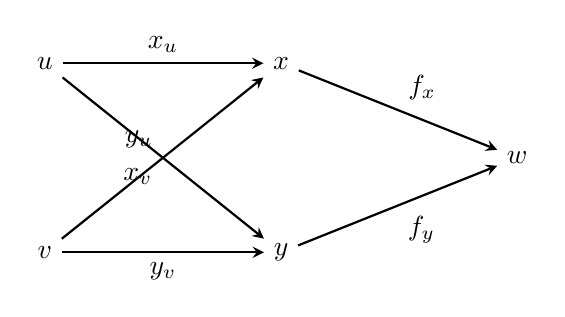
\begin{tikzpicture}[scale=1.0, >=stealth]
    \node (u) at (0,1.2) {\(u\)};
    \node (v) at (0,-1.2) {\(v\)};
    \node (x) at (3,1.2) {\(x\)};
    \node (y) at (3,-1.2) {\(y\)};
    \node (w) at (6,0) {\(w\)};

    \draw[->, thick] (u) -- (x) node[midway, above] {\(x_u\)};
    \draw[->, thick] (v) -- (x) node[midway, below left] {\(x_v\)};
    \draw[->, thick] (u) -- (y) node[midway, above left] {\(y_u\)};
    \draw[->, thick] (v) -- (y) node[midway, below] {\(y_v\)};

    \draw[->, thick] (x) -- (w) node[midway, above right] {\(f_x\)};
    \draw[->, thick] (y) -- (w) node[midway, below right] {\(f_y\)};
\end{tikzpicture}
\caption{Each path from an input variable to \(w\) contributes one product of
derivatives.}
\end{figure}

To find \(w_u\), add the products along all paths from \(u\) to \(w\):
\[
\boxed{
    w_u=f_xx_u+f_yy_u.
}
\]
To find \(w_v\), add the products along all paths from \(v\) to \(w\):
\[
\boxed{
    w_v=f_xx_v+f_yy_v.
}
\]

These two formulas are one matrix product.  The Jacobian of
\[
    f:\mathbb R^2\to\mathbb R
\]
is the row matrix
\[
    J_f(x,y)=
    \begin{pmatrix}
        f_x & f_y
    \end{pmatrix}.
\]
The Jacobian of
\[
    G(u,v)=(x(u,v),y(u,v))
\]
is
\[
    J_G(u,v)
    =
    \begin{pmatrix}
        x_u & x_v\\
        y_u & y_v
    \end{pmatrix}.
\]
Therefore
\[
    J_{f\circ G}(u,v)
    =
    \begin{pmatrix}
        f_x & f_y
    \end{pmatrix}
    \begin{pmatrix}
        x_u & x_v\\
        y_u & y_v
    \end{pmatrix}
    =
    \begin{pmatrix}
        f_xx_u+f_yy_u
        &
        f_xx_v+f_yy_v
    \end{pmatrix}.
\]

\begin{example}[A dependency diagram calculation]
Let
\[
    w=x^2+xy,
\]
where
\[
    x=u+v^2,
    \qquad
    y=uv.
\]
Find \(w_u\) and \(w_v\) at
\[
    (u,v)=(2,1).
\]

First compute the intermediate values:
\[
    x(2,1)=2+1=3,
    \qquad
    y(2,1)=2.
\]
The partial derivatives of \(w\) are
\[
    w_x=2x+y,
    \qquad
    w_y=x.
\]
At \((x,y)=(3,2)\),
\[
    w_x=8,
    \qquad
    w_y=3.
\]

The derivatives of the intermediate variables are
\[
    x_u=1,
    \qquad
    x_v=2v,
\]
and
\[
    y_u=v,
    \qquad
    y_v=u.
\]
At \((u,v)=(2,1)\),
\[
    x_u=1,
    \qquad
    x_v=2,
    \qquad
    y_u=1,
    \qquad
    y_v=2.
\]
Thus
\[
\begin{aligned}
    w_u
    &=
    w_xx_u+w_yy_u\\
    &=
    8(1)+3(1)\\
    &=
    11,
\end{aligned}
\]
and
\[
\begin{aligned}
    w_v
    &=
    w_xx_v+w_yy_v\\
    &=
    8(2)+3(2)\\
    &=
    22.
\end{aligned}
\]
\end{example}

\subsection{The chain rule as ``linearize, then compose''}

The matrix formula can look like a bookkeeping rule:
\[
    J_{F\circ G}=J_FJ_G.
\]
But the meaning is more geometric.

A small input displacement
\[
    \Delta\mathbf u
\]
first passes through the best linear approximation to \(G\):
\[
    \Delta\mathbf x\approx J_G(\mathbf p)\Delta\mathbf u.
\]
Then that output displacement passes through the best linear approximation to \(F\):
\[
    \Delta\mathbf z
    \approx
    J_F(G(\mathbf p))\Delta\mathbf x.
\]
Substitute the first approximation into the second:
\[
    \Delta\mathbf z
    \approx
    J_F(G(\mathbf p))J_G(\mathbf p)\Delta\mathbf u.
\]
So the chain rule says:
\[
\boxed{
    \text{linearize each map, then compose the linearizations.}
}
\]

\begin{figure}[h]
\centering
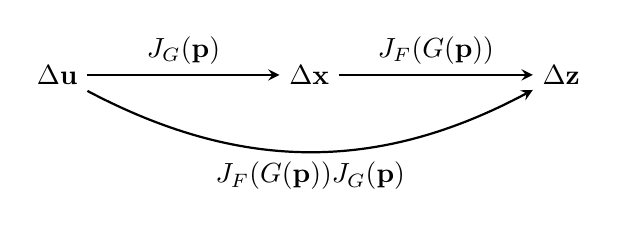
\begin{tikzpicture}[scale=1.0, >=stealth]
    \node (du) at (0,0) {\(\Delta\mathbf u\)};
    \node (dx) at (3.2,0) {\(\Delta\mathbf x\)};
    \node (dz) at (6.4,0) {\(\Delta\mathbf z\)};

    \draw[->, thick] (du) -- (dx)
        node[midway, above] {\(J_G(\mathbf p)\)};
    \draw[->, thick] (dx) -- (dz)
        node[midway, above] {\(J_F(G(\mathbf p))\)};

    \draw[->, thick, bend right=28] (du) to
        node[midway, below] {\(J_F(G(\mathbf p))J_G(\mathbf p)\)}
        (dz);
\end{tikzpicture}
\caption{The derivative of a composition is the composition of the derivatives.}
\end{figure}

There is a cleaner notation hiding inside the matrix multiplication.  If
\[
    x=x(u,v)
    \qquad\text{and}\qquad
    y=y(u,v),
\]
then their differentials are
\[
    dx=x_u\,du+x_v\,dv,
    \qquad
    dy=y_u\,du+y_v\,dv.
\]
Substituting these into
\[
    df=f_x\,dx+f_y\,dy
\]
produces the same chain rule formulas.  That substitution looks almost too simple.
It is not a trick.  It is the beginning of the pullback idea for differential forms, and it
will become one of the quiet engines behind line integrals, surface integrals, and the
integral theorems later in the book.
% Draft follows the Chapter 8 outline for Sections 8.3 and 8.4, and continues
% the Chapter 7 differential/Jacobian thread. :contentReference[oaicite:0]{index=0} :contentReference[oaicite:1]{index=1} :contentReference[oaicite:2]{index=2}

\section{Differentials and the chain rule}
\label{sec:8.3}

Section \ref{sec:8.2} wrote the chain rule as a matrix product:
\[
    J_{F\circ G}=J_FJ_G.
\]
That is the right language for transformations.  But Section \ref{sec:7.4} gave us
another language for the same linear idea:
\[
    df=f_x\,dx+f_y\,dy.
\]
The chain rule becomes especially clean when we substitute one differential into another.

\subsection{Substitution into differentials}

Return to the greenhouse temperature field from Section \ref{sec:8.1}:
\[
    T(x,y)=20+3x-y-\frac12x^2-\frac14y^2.
\]
Its differential is
\[
    dT=(3-x)\,dx+\left(-1-\frac12y\right)\,dy.
\]

Now suppose the greenhouse floor is being described by a slanted coordinate grid
\((u,v)\), where
\[
    x=1+u+2v,
    \qquad
    y=2+u-v.
\]
The point \((u,v)=(0,0)\) corresponds to
\[
    (x,y)=(1,2).
\]
The temperature as a function of the grid coordinates is
\[
    A(u,v)=T(1+u+2v,\;2+u-v).
\]

We could expand \(A(u,v)\) and differentiate.  But the differential does the same work
without expanding.

First,
\[
    dx=d(1+u+2v)=du+2\,dv,
\]
and
\[
    dy=d(2+u-v)=du-dv.
\]
At \((x,y)=(1,2)\),
\[
    dT_{(1,2)}
    =
    2\,dx-2\,dy.
\]
Substitute the expressions for \(dx\) and \(dy\):
\[
\begin{aligned}
    dA_{(0,0)}
    &=
    2(du+2\,dv)-2(du-dv)\\
    &=
    6\,dv.
\end{aligned}
\]
So, at the center point of this grid,
\[
    A_u(0,0)=0,
    \qquad
    A_v(0,0)=6.
\]
A tiny step in the \(u\)-direction does not change temperature to first order.  A tiny
step in the \(v\)-direction raises the temperature at rate \(6\).

The same computation works away from the point.  Since
\[
    dT=(3-x)\,dx+\left(-1-\frac12y\right)\,dy,
\]
and
\[
    dx=du+2\,dv,
    \qquad
    dy=du-dv,
\]
we get
\[
\begin{aligned}
    dA
    &=
    (3-x)(du+2\,dv)
    +
    \left(-1-\frac12y\right)(du-dv)\\
    &=
    \left(2-x-\frac12y\right)du
    +
    \left(7-2x+\frac12y\right)dv,
\end{aligned}
\]
where
\[
    x=1+u+2v,
    \qquad
    y=2+u-v.
\]
Thus
\[
    A_u=
    2-x-\frac12y,
    \qquad
    A_v=
    7-2x+\frac12y.
\]
This is the chain rule written as substitution into differentials.

\subsection{The general substitution rule}

Let
\[
    z=f(x,y),
\]
where
\[
    x=x(u,v),
    \qquad
    y=y(u,v).
\]
Then
\[
    z=f(x(u,v),y(u,v)).
\]
The differential of \(f\) is
\[
    df=f_x\,dx+f_y\,dy.
\]
The intermediate coordinates have differentials
\[
    dx=x_u\,du+x_v\,dv,
\]
and
\[
    dy=y_u\,du+y_v\,dv.
\]
Substitute:
\[
\begin{aligned}
    dz
    &=
    f_x(x_u\,du+x_v\,dv)
    +
    f_y(y_u\,du+y_v\,dv)\\
    &=
    (f_xx_u+f_yy_u)\,du
    +
    (f_xx_v+f_yy_v)\,dv.
\end{aligned}
\]
Therefore
\[
\boxed{
    \frac{\partial z}{\partial u}
    =
    f_x\frac{\partial x}{\partial u}
    +
    f_y\frac{\partial y}{\partial u},
}
\]
and
\[
\boxed{
    \frac{\partial z}{\partial v}
    =
    f_x\frac{\partial x}{\partial v}
    +
    f_y\frac{\partial y}{\partial v}.
}
\]
The partial derivatives \(f_x\) and \(f_y\) are evaluated at
\[
    (x(u,v),y(u,v)).
\]

This is the same chain rule as Section \ref{sec:8.2}.  In matrix form,
\[
    \begin{pmatrix}
        z_u & z_v
    \end{pmatrix}
    =
    \begin{pmatrix}
        f_x & f_y
    \end{pmatrix}
    \begin{pmatrix}
        x_u & x_v\\
        y_u & y_v
    \end{pmatrix}.
\]
In differential form,
\[
    dz=f_x\,dx+f_y\,dy,
\]
with
\[
    dx=x_u\,du+x_v\,dv,
    \qquad
    dy=y_u\,du+y_v\,dv.
\]
The two statements are the same linear map, written in two dialects.

\begin{theorem}[Chain rule for differentials]
Let
\[
    G:U\subseteq\mathbb R^k\to\mathbb R^n
\]
be differentiable at \(\mathbf p\), and let
\[
    f:V\subseteq\mathbb R^n\to\mathbb R
\]
be differentiable at \(G(\mathbf p)\), with \(G(U)\subseteq V\).  Then
\[
    f\circ G
\]
is differentiable at \(\mathbf p\), and
\[
\boxed{
    d(f\circ G)_{\mathbf p}
    =
    df_{G(\mathbf p)}\circ DG(\mathbf p).
}
\]
Equivalently, for every small input displacement \(\mathbf h\),
\[
\boxed{
    d(f\circ G)_{\mathbf p}(\mathbf h)
    =
    df_{G(\mathbf p)}\bigl(DG(\mathbf p)\mathbf h\bigr).
}
\]
\end{theorem}

\begin{proof}
This is the matrix chain rule from Section \ref{sec:8.2}, with the outer map scalar-valued.
The derivative of \(G\) sends an input displacement \(\mathbf h\) to the predicted
displacement in the intermediate space.  The differential \(df\) then eats that predicted
intermediate displacement and returns the predicted change in \(f\).  Thus the first-order
change of the composition is
\[
    df_{G(\mathbf p)}\circ DG(\mathbf p).
\]
\end{proof}

\subsection{Why \texorpdfstring{\(du=u_x\,dx+u_y\,dy\)}{du = ux dx + uy dy} behaves naturally}

The notation
\[
    du=u_x\,dx+u_y\,dy
\]
can look suspicious the first time we see it.  It helps to remember what \(du\) is:
the differential of the function \(u(x,y)\).

For example, define new coordinate readings
\[
    u=x+2y,
    \qquad
    v=x-y.
\]
Then
\[
    du=dx+2\,dy,
\]
and
\[
    dv=dx-dy.
\]
These equations say how the new coordinate readings change when the old point moves.

Now solve for \(x\) and \(y\):
\[
    x=\frac{u+2v}{3},
    \qquad
    y=\frac{u-v}{3}.
\]
So
\[
    dx=\frac13\,du+\frac23\,dv,
\]
and
\[
    dy=\frac13\,du-\frac13\,dv.
\]
Substitute these into the formula for \(du\):
\[
\begin{aligned}
    dx+2\,dy
    &=
    \left(\frac13\,du+\frac23\,dv\right)
    +
    2\left(\frac13\,du-\frac13\,dv\right)\\
    &=
    du.
\end{aligned}
\]
The notation checks itself.

The reason is not algebraic luck.  The symbol \(d\) means ``take the linear part.''
Linear parts compose cleanly, so their coordinate formulas substitute cleanly.

\subsection{Pullback preview: moving formulas to parameter space}

A \(1\)-form in the plane has the shape
\[
    \omega=P(x,y)\,dx+Q(x,y)\,dy.
\]
A parametrization or coordinate change
\[
    G(u,v)=(x(u,v),y(u,v))
\]
moves this form to the \((u,v)\)-plane by substituting:
\[
\boxed{
    G^*\omega
    =
    P(x(u,v),y(u,v))\,d(x(u,v))
    +
    Q(x(u,v),y(u,v))\,d(y(u,v)).
}
\]
This new \(1\)-form
\[
    G^*\omega
\]
is called the \emph{pullback} of \(\omega\) by \(G\).

The name sounds abstract, but the action is concrete: replace \(x,y,dx,dy\) by their
expressions in the new variables.

\begin{example}[Pulling the swirl form into polar coordinates]
Consider the swirling \(1\)-form
\[
    \omega=-y\,dx+x\,dy.
\]
Use the polar coordinate map
\[
    G(r,\theta)=(r\cos\theta,r\sin\theta).
\]
Then
\[
    x=r\cos\theta,
    \qquad
    y=r\sin\theta.
\]
Also,
\[
    dx=\cos\theta\,dr-r\sin\theta\,d\theta,
\]
and
\[
    dy=\sin\theta\,dr+r\cos\theta\,d\theta.
\]
Substitute into \(\omega\):
\[
\begin{aligned}
G^*\omega
&=
-r\sin\theta(\cos\theta\,dr-r\sin\theta\,d\theta)
+
r\cos\theta(\sin\theta\,dr+r\cos\theta\,d\theta)\\
&=
(-r\sin\theta\cos\theta+r\cos\theta\sin\theta)\,dr\\
&\qquad
+
r^2(\sin^2\theta+\cos^2\theta)\,d\theta\\
&=
r^2\,d\theta.
\end{aligned}
\]
So
\[
\boxed{
    G^*(-y\,dx+x\,dy)=r^2\,d\theta.
}
\]
The trigonometry disappeared.  In polar coordinates, the swirl form simply measures
angular motion, weighted by \(r^2\).
\end{example}

This is the first real glimpse of why differential forms fit coordinate changes so well.
They are built to be substituted into.

\subsection{When substitution breaks}

The differentiability condition is not cosmetic.  If the coordinate map has a corner,
there may be no linear part to substitute.

Let
\[
    G(u)=(|u|,0),
\]
and take the \(1\)-form
\[
    \omega=dx.
\]
For \(u>0\),
\[
    x=|u|=u,
\]
so
\[
    G^*\omega=du.
\]
For \(u<0\),
\[
    x=|u|=-u,
\]
so
\[
    G^*\omega=-du.
\]
At \(u=0\), the function
\[
    |u|
\]
has no derivative.  Therefore \(d|u|\) does not exist at \(0\), and the pullback of
\(dx\) is not defined there.

This is the same warning as the chain rule along a curve:
\[
    \text{no differentiability}
    \quad\Longrightarrow\quad
    \text{no dependable first-order substitution.}
\]

The outer function also has to be differentiable.  If we try to substitute a fake
``differential'' made only from partial derivatives at a point where no total derivative
exists, the same counterexamples from Sections \ref{sec:8.1} and \ref{sec:8.2} return.
The differential is the total derivative, not a list of coordinate slopes.

\subsection{A first look at coordinate-free notation}

The pullback formula lets us write the chain rule in a short form:
\[
\boxed{
    d(f\circ G)=G^*(df).
}
\]
Read it from right to left.

First take the differential of \(f\) in the \(x\)-space:
\[
    df.
\]
Then pull that differential back through the map \(G\) into the input space:
\[
    G^*(df).
\]
The result is the differential of the composite:
\[
    d(f\circ G).
\]

This notation hides the coordinates, but it does not hide the computation.  If
\[
    G(u,v)=(x(u,v),y(u,v)),
\]
then
\[
    G^*(df)
    =
    f_x(x(u,v),y(u,v))\,dx
    +
    f_y(x(u,v),y(u,v))\,dy,
\]
where
\[
    dx=x_u\,du+x_v\,dv,
    \qquad
    dy=y_u\,du+y_v\,dv.
\]
Expanding gives the familiar chain rule.

The notation
\[
    d(f\circ G)=G^*(df)
\]
says the same thing without committing to the names of the coordinates.  That will
matter more and more as we integrate forms over curves and surfaces.

The pullback of the swirl form by polar coordinates gave
\[
    -y\,dx+x\,dy
    \quad\longmapsto\quad
    r^2\,d\theta.
\]
That little simplification is a hint.  Some problems are hard only because the coordinates
are poorly matched to the geometry.  Polar, cylindrical, and spherical coordinates are
not new calculus rules.  They are coordinate changes, and the chain rule tells us exactly
how derivatives and differentials move through them.

\section{Coordinate changes}
\label{sec:8.4}

Section \ref{sec:8.3} treated a coordinate change as a differentiable map and moved
differentials through it by substitution.  Now we use that idea on the coordinate systems
from Chapter \ref{ch:4}: polar, cylindrical, and spherical coordinates.

A coordinate change does two things at once.  It gives new labels to points, and it
stretches small pieces of length, area, and volume.  The chain rule handles the labels.
The Jacobian determinant measures the stretching.

\subsection{Polar coordinates and the chain rule}

The polar coordinate map is
\[
    G(r,\theta)=(x,y)=(r\cos\theta,r\sin\theta).
\]
If
\[
    f=f(x,y),
\]
then the same scalar field written in polar coordinates is
\[
    F(r,\theta)=f(r\cos\theta,r\sin\theta).
\]

Take differentials:
\[
    dx=\cos\theta\,dr-r\sin\theta\,d\theta,
\]
and
\[
    dy=\sin\theta\,dr+r\cos\theta\,d\theta.
\]
Since
\[
    df=f_x\,dx+f_y\,dy,
\]
substitution gives
\[
\begin{aligned}
dF
&=
f_x(\cos\theta\,dr-r\sin\theta\,d\theta)
+
f_y(\sin\theta\,dr+r\cos\theta\,d\theta)\\
&=
(f_x\cos\theta+f_y\sin\theta)\,dr
+
(-rf_x\sin\theta+rf_y\cos\theta)\,d\theta.
\end{aligned}
\]
Therefore
\[
\boxed{
    F_r=f_x\cos\theta+f_y\sin\theta,
}
\]
and
\[
\boxed{
    F_\theta=-r f_x\sin\theta+r f_y\cos\theta.
}
\]
The partial derivatives \(f_x\) and \(f_y\) are evaluated at
\[
    (x,y)=(r\cos\theta,r\sin\theta).
\]

\begin{example}[Temperature around a circular fountain]
A circular fountain sits at the origin.  A temperature field on the stone plaza is
\[
    T(x,y)=20+\frac{6}{1+x^2+y^2}+x-2y.
\]
The term
\[
    \frac{6}{1+x^2+y^2}
\]
is strongest near the fountain.  The term \(x-2y\) tilts the temperature field across
the plaza.

In polar coordinates,
\[
\begin{aligned}
A(r,\theta)
&=
T(r\cos\theta,r\sin\theta)\\
&=
20+\frac{6}{1+r^2}+r\cos\theta-2r\sin\theta.
\end{aligned}
\]
Differentiate directly:
\[
    A_r
    =
    -\frac{12r}{(1+r^2)^2}+\cos\theta-2\sin\theta,
\]
and
\[
    A_\theta
    =
    -r\sin\theta-2r\cos\theta.
\]

At the point
\[
    r=2,
    \qquad
    \theta=\frac{\pi}{2},
\]
we are at
\[
    (x,y)=(0,2).
\]
There,
\[
    A_r
    =
    -\frac{24}{25}-2
    =
    -\frac{74}{25},
\]
and
\[
    A_\theta=-2.
\]
The first number is a rate per meter in the radial direction.  The second is a rate per
radian, not per meter.  At radius \(2\), one radian of angular motion has length \(2\).
So the tangential rate per meter is
\[
    \frac{A_\theta}{r}=\frac{-2}{2}=-1.
\]
This distinction is where many polar-coordinate mistakes begin: an angle is not a
length.
\end{example}

\begin{figure}[h]
\centering
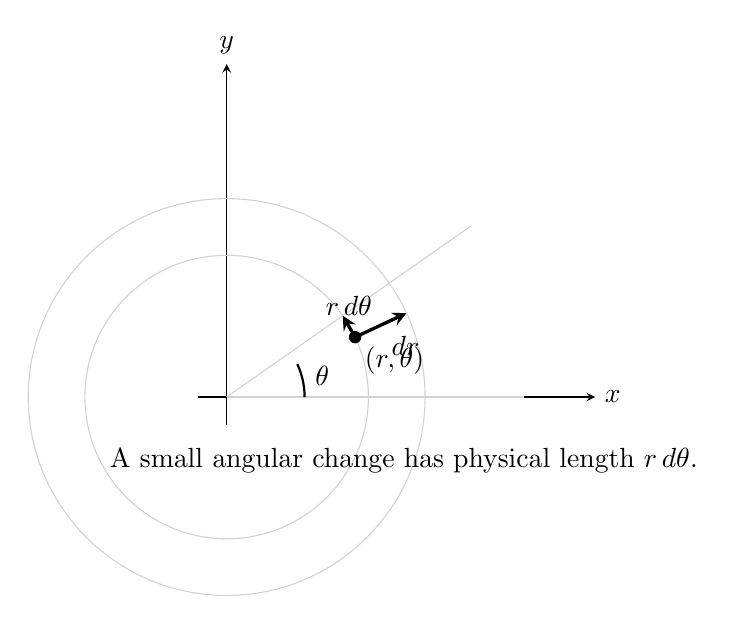
\begin{tikzpicture}[scale=0.9, >=stealth]
    \draw[->] (-0.4,0) -- (5.2,0) node[right] {\(x\)};
    \draw[->] (0,-0.4) -- (0,4.7) node[above] {\(y\)};

    \draw[gray!35] (0,0) circle (2);
    \draw[gray!35] (0,0) circle (2.8);
    \draw[gray!35] (0,0) -- (4.2,0);
    \draw[gray!35] (0,0) -- ({4.2*cos(35)}, {4.2*sin(35)});

    \coordinate (P) at ({2*cos(25)}, {2*sin(25)});
    \coordinate (Pr) at ({2.8*cos(25)}, {2.8*sin(25)});
    \coordinate (Pt) at ({2*cos(35)}, {2*sin(35)});

    \fill (P) circle (2.5pt);
    \node[below right] at (P) {\((r,\theta)\)};

    \draw[->, very thick] (P) -- (Pr) node[midway, below right] {\(dr\)};
    \draw[->, very thick] (P) -- (Pt) node[midway, above] {\(r\,d\theta\)};

    \draw[thick] (1.1,0) arc[start angle=0,end angle=25,radius=1.1];
    \node at (1.35,0.3) {\(\theta\)};

    \node at (2.5,-0.9) {A small angular change has physical length \(r\,d\theta\).};
\end{tikzpicture}
\caption{In polar coordinates, radial and angular changes have different length scales.}
\end{figure}

\subsection{Cylindrical coordinates}

Cylindrical coordinates are polar coordinates with height:
\[
    x=r\cos\theta,
    \qquad
    y=r\sin\theta,
    \qquad
    z=z.
\]
If
\[
    f=f(x,y,z),
\]
write
\[
    F(r,\theta,z)=f(r\cos\theta,r\sin\theta,z).
\]
The differentials are
\[
    dx=\cos\theta\,dr-r\sin\theta\,d\theta,
\]
\[
    dy=\sin\theta\,dr+r\cos\theta\,d\theta,
\]
and
\[
    dz=dz.
\]
Substituting into
\[
    df=f_x\,dx+f_y\,dy+f_z\,dz
\]
gives
\[
\boxed{
    F_r=f_x\cos\theta+f_y\sin\theta,
}
\]
\[
\boxed{
    F_\theta=-r f_x\sin\theta+r f_y\cos\theta,
}
\]
and
\[
\boxed{
    F_z=f_z.
}
\]

\begin{example}[Pressure inside a round tank]
A round tank has pressure field
\[
    p(x,y,z)=100-z+xy.
\]
In cylindrical coordinates,
\[
    xy=(r\cos\theta)(r\sin\theta)=r^2\sin\theta\cos\theta.
\]
So
\[
    P(r,\theta,z)=100-z+r^2\sin\theta\cos\theta.
\]
Then
\[
    P_r=2r\sin\theta\cos\theta,
\]
\[
    P_\theta=r^2(\cos^2\theta-\sin^2\theta),
\]
and
\[
    P_z=-1.
\]
The derivative \(P_z=-1\) says pressure drops by one unit per meter of height.  The
derivative \(P_\theta\) is a rate per radian around the tank.  To convert it to a rate per
meter along a circular ring, divide by \(r\).
\end{example}

\subsection{Spherical coordinates}

Chapter \ref{ch:4} used the spherical coordinates
\[
    (\rho,\theta,\phi),
\]
where \(\rho\) is distance from the origin, \(\theta\) is the angle around the \(z\)-axis,
and \(\phi\) is the angle down from the positive \(z\)-axis.  The conversion formulas are
\[
\boxed{
    x=\rho\sin\phi\cos\theta,\qquad
    y=\rho\sin\phi\sin\theta,\qquad
    z=\rho\cos\phi.
}
\]

Let
\[
    F(\rho,\theta,\phi)
    =
    f(\rho\sin\phi\cos\theta,\rho\sin\phi\sin\theta,\rho\cos\phi).
\]
The chain rule gives
\[
\boxed{
F_\rho
=
f_x\sin\phi\cos\theta
+
f_y\sin\phi\sin\theta
+
f_z\cos\phi.
}
\]
The \(\theta\)-derivative is
\[
\boxed{
F_\theta
=
-\rho f_x\sin\phi\sin\theta
+
\rho f_y\sin\phi\cos\theta.
}
\]
The \(\phi\)-derivative is
\[
\boxed{
F_\phi
=
\rho f_x\cos\phi\cos\theta
+
\rho f_y\cos\phi\sin\theta
-
\rho f_z\sin\phi.
}
\]
Again, the partial derivatives \(f_x,f_y,f_z\) are evaluated at the rectangular point
corresponding to \((\rho,\theta,\phi)\).

The length scales are different:
\[
\begin{array}{c|c}
\text{coordinate change} & \text{physical length} \\ \hline
d\rho & d\rho\\[1mm]
d\theta & \rho\sin\phi\,d\theta\\[1mm]
d\phi & \rho\,d\phi
\end{array}
\]
A small change in \(\theta\) moves around a horizontal circle of radius
\[
    \rho\sin\phi.
\]
A small change in \(\phi\) moves along a meridian of radius
\[
    \rho.
\]

\begin{example}[A radially symmetric field]
Let
\[
    f(x,y,z)=\frac{1}{1+x^2+y^2+z^2}.
\]
Since
\[
    x^2+y^2+z^2=\rho^2,
\]
the spherical form is
\[
    F(\rho,\theta,\phi)=\frac{1}{1+\rho^2}.
\]
Therefore
\[
    F_\rho=-\frac{2\rho}{(1+\rho^2)^2},
\]
while
\[
    F_\theta=0,
    \qquad
    F_\phi=0.
\]
In spherical coordinates the symmetry is visible: the field changes only when we move
toward or away from the origin.  Moving around a sphere of fixed \(\rho\) does not
change the value.
\end{example}

\subsection{Gradients in non-Cartesian coordinates}

The differential
\[
    df
\]
does not care which coordinates we use.  But the gradient vector does care about
lengths, because it measures change per unit distance.

In polar coordinates,
\[
    dF=F_r\,dr+F_\theta\,d\theta.
\]
The radial coordinate \(r\) is a distance.  The angular coordinate \(\theta\) is not.  A
change \(d\theta\) at radius \(r\) has physical length \(r\,d\theta\).

Let
\[
    \mathbf e_r=(\cos\theta,\sin\theta),
    \qquad
    \mathbf e_\theta=(-\sin\theta,\cos\theta).
\]
Then, away from the origin,
\[
\boxed{
    \nabla f
    =
    F_r\,\mathbf e_r
    +
    \frac{1}{r}F_\theta\,\mathbf e_\theta.
}
\]
The factor
\[
    \frac1r
\]
appears because \(F_\theta\) is change per radian, while the gradient needs change per
unit length.

In cylindrical coordinates,
\[
\boxed{
    \nabla f
    =
    F_r\,\mathbf e_r
    +
    \frac1rF_\theta\,\mathbf e_\theta
    +
    F_z\,\mathbf k,
    \qquad r>0.
}
\]

In spherical coordinates, define the unit vectors
\[
    \mathbf e_\rho
    =
    (\sin\phi\cos\theta,\sin\phi\sin\theta,\cos\phi),
\]
\[
    \mathbf e_\theta
    =
    (-\sin\theta,\cos\theta,0),
\]
and
\[
    \mathbf e_\phi
    =
    (\cos\phi\cos\theta,\cos\phi\sin\theta,-\sin\phi).
\]
Then, away from the origin and away from the \(z\)-axis,
\[
\boxed{
    \nabla f
    =
    F_\rho\,\mathbf e_\rho
    +
    \frac{1}{\rho\sin\phi}F_\theta\,\mathbf e_\theta
    +
    \frac1\rho F_\phi\,\mathbf e_\phi.
}
\]
The denominators are the length scales:
\[
    d\rho,\qquad
    \rho\sin\phi\,d\theta,\qquad
    \rho\,d\phi.
\]

These formulas should not be memorized as disconnected rules.  They come from one
sentence:

\[
    \text{differentiate with respect to a coordinate, then divide by the physical length of
    that coordinate step.}
\]

\subsection{Local stretching and the Jacobian determinant}

A coordinate change does not only change derivatives.  It also changes tiny areas and
volumes.

For polar coordinates,
\[
    x=r\cos\theta,
    \qquad
    y=r\sin\theta.
\]
We already found
\[
    dx=\cos\theta\,dr-r\sin\theta\,d\theta,
\]
and
\[
    dy=\sin\theta\,dr+r\cos\theta\,d\theta.
\]
Take the wedge product:
\[
\begin{aligned}
dx\wedge dy
&=
(\cos\theta\,dr-r\sin\theta\,d\theta)
\wedge
(\sin\theta\,dr+r\cos\theta\,d\theta)\\
&=
r\cos^2\theta\,dr\wedge d\theta
+
r\sin^2\theta\,dr\wedge d\theta\\
&=
r\,dr\wedge d\theta.
\end{aligned}
\]
Thus
\[
\boxed{
    dx\wedge dy=r\,dr\wedge d\theta.
}
\]
The factor \(r\) is the Jacobian determinant:
\[
\boxed{
    \frac{\partial(x,y)}{\partial(r,\theta)}
    =
    \det
    \begin{pmatrix}
        \cos\theta & -r\sin\theta\\
        \sin\theta & r\cos\theta
    \end{pmatrix}
    =
    r.
}
\]
A tiny polar rectangle with side lengths \(dr\) and \(d\theta\) maps to a tiny sector
whose area is approximately
\[
    r\,dr\,d\theta.
\]

For cylindrical coordinates,
\[
    x=r\cos\theta,
    \qquad
    y=r\sin\theta,
    \qquad
    z=z.
\]
The volume form becomes
\[
\boxed{
    dx\wedge dy\wedge dz
    =
    r\,dr\wedge d\theta\wedge dz.
}
\]
So the local volume stretching factor is
\[
\boxed{
    r.
}
\]

For spherical coordinates in the order
\[
    (\rho,\theta,\phi),
\]
the Jacobian determinant is
\[
\boxed{
    \frac{\partial(x,y,z)}{\partial(\rho,\theta,\phi)}
    =
    -\rho^2\sin\phi.
}
\]
The negative sign is an orientation sign.  It says that the ordered coordinate directions
\[
    (\rho,\theta,\phi)
\]
have the opposite orientation from
\[
    (x,y,z).
\]
The size of the local volume stretching is
\[
\boxed{
    \rho^2\sin\phi.
}
\]
Equivalently,
\[
\boxed{
    dx\wedge dy\wedge dz
    =
    -\rho^2\sin\phi\,
    d\rho\wedge d\theta\wedge d\phi.
}
\]
If we order the spherical coordinates as
\[
    (\rho,\phi,\theta),
\]
then the sign becomes positive:
\[
\boxed{
    dx\wedge dy\wedge dz
    =
    \rho^2\sin\phi\,
    d\rho\wedge d\phi\wedge d\theta.
}
\]

The absolute value is what appears in ordinary volume computations:
\[
    dV=\rho^2\sin\phi\,d\rho\,d\phi\,d\theta.
\]
The wedge product keeps the orientation information too.

\subsection{Where coordinates fail}

Coordinate changes have their own weak spots.

In polar coordinates,
\[
    (r,\theta)
\]
and
\[
    (r,\theta+2\pi)
\]
describe the same point.  At the origin, the problem is stronger:
\[
    (0,\theta)
\]
describes the origin for every \(\theta\).  The angle is meaningless there.

The Jacobian determinant detects this:
\[
    \frac{\partial(x,y)}{\partial(r,\theta)}=r.
\]
At
\[
    r=0,
\]
the determinant is \(0\).  A small angular change at the origin produces no physical
motion at all.

The gradient formula also warns us:
\[
    \nabla f
    =
    F_r\,\mathbf e_r+\frac1rF_\theta\,\mathbf e_\theta.
\]
At \(r=0\), the factor \(1/r\) is not defined.  The failure belongs to the coordinates,
not necessarily to the function.

\begin{example}[A smooth function in bad coordinates]
Let
\[
    f(x,y)=x.
\]
This is as smooth as a function can be.  In polar coordinates,
\[
    F(r,\theta)=r\cos\theta.
\]
At \(r=0\),
\[
    F(0,\theta)=0
\]
for every \(\theta\).  The same physical point has infinitely many coordinate names.
So we should not expect polar coordinates to give a single clean coordinate description
of the derivative at the origin.

The rectangular gradient is simple:
\[
    \nabla f=(1,0).
\]
The polar description breaks because the coordinate system breaks.
\end{example}

Spherical coordinates have the same kind of singular sets.  At
\[
    \rho=0,
\]
both angles lose meaning.  On the positive and negative \(z\)-axis,
\[
    \sin\phi=0,
\]
so the angle \(\theta\) loses meaning.  The stretching factor
\[
    \rho^2\sin\phi
\]
vanishes there.

A coordinate system is a tool, not part of the space itself.  When its Jacobian determinant
is nonzero, the tool behaves locally like a reversible linear map.  When the determinant
vanishes, something has collapsed: an angle, an area, a volume, or a direction.

That observation is too sharp to leave alone.  If a transformation has a nonzero Jacobian
determinant at a point, should it have a local inverse nearby?  The polar map away from
the origin says yes.  The origin says no.  The next question is to turn that pattern into a
theorem about inverse functions.
% Draft follows the Chapter 8 outline for Sections 8.5 and 8.6, especially the
% inverse-function and implicit-function entries. :contentReference[oaicite:0]{index=0} :contentReference[oaicite:1]{index=1}
% It also continues the Chapter 7 Jacobian/differential thread. :contentReference[oaicite:2]{index=2}

\section{Inverse functions}
\label{sec:8.5}

Section \ref{sec:8.4} ended with a sharp clue.  A coordinate map behaves well when
its Jacobian determinant is nonzero, and it breaks where the determinant vanishes.
Polar coordinates gave the simplest example:
\[
    x=r\cos\theta,\qquad y=r\sin\theta,
\]
with
\[
    \frac{\partial(x,y)}{\partial(r,\theta)}=r.
\]
Away from the origin, the map behaves locally like a reversible change of coordinates.
At the origin, all angles collapse to the same point.

That raises the question this section answers:

\[
    \text{When can we solve locally for the inputs from the outputs?}
\]

\subsection{What it means to solve locally for inputs from outputs}

A tracking camera sees the position of a small robot on a floor.  The robot's internal
coordinates are \((u,v)\), but the camera reports the floor coordinates \((x,y)\).  Suppose
the conversion is
\[
    F(u,v)=(x,y)=(e^u\cos v,\ e^u\sin v).
\]
This is a polar-type map.  The coordinate \(u\) controls distance from the origin, since
\[
    \sqrt{x^2+y^2}=e^u,
\]
and \(v\) controls angle.

Take
\[
    (u,v)=\left(\ln 2,\frac{\pi}{6}\right).
\]
Then
\[
    F\left(\ln 2,\frac{\pi}{6}\right)
    =
    \left(2\cdot\frac{\sqrt3}{2},\ 2\cdot\frac12\right)
    =
    (\sqrt3,1).
\]
If the camera reports
\[
    (x,y)=(\sqrt3,1),
\]
then the internal coordinates near this point are
\[
    u=\ln\sqrt{x^2+y^2},
\]
and
\[
    v=\Arg(x+iy),
\]
where \(\Arg\) is chosen as the angle branch near \(\pi/6\).  So near
\[
    (\sqrt3,1),
\]
we can recover
\[
    (u,v)
\]
from
\[
    (x,y).
\]

But there is an immediate catch:
\[
    F(u,v+2\pi)=F(u,v).
\]
So \(F\) is not one-to-one on the whole \((u,v)\)-plane.  The same floor point has
many angle names.  Still, if we zoom in near
\[
    \left(\ln2,\frac{\pi}{6}\right),
\]
there is no ambiguity.  Nearby outputs come from one nearby input.

That is what \emph{local inverse} means.

\begin{definition}[Local inverse]
Let
\[
    F:D\subseteq\mathbb R^n\to\mathbb R^n
\]
and let
\[
    \mathbf p\in D.
\]
A function \(G\) is a \emph{local inverse} of \(F\) near \(\mathbf p\) if there are
neighborhoods \(U\) of \(\mathbf p\) and \(V\) of \(F(\mathbf p)\) such that
\[
    F:U\to V
\]
is one-to-one and onto, and
\[
    G:V\to U
\]
satisfies
\[
    G(F(\mathbf x))=\mathbf x
    \quad\text{for all }\mathbf x\in U,
\]
and
\[
    F(G(\mathbf y))=\mathbf y
    \quad\text{for all }\mathbf y\in V.
\]
\end{definition}

The word \emph{local} matters.  A map can have a local inverse near each point and
still fail to have one global inverse.

\subsection{The derivative of an inverse transformation}

The inverse map does not only exist locally.  Its derivative is forced by the chain rule.

Let
\[
    \mathbf q=F(\mathbf p),
\]
and suppose
\[
    G=F^{-1}
\]
near \(\mathbf q\).  Then
\[
    G(F(\mathbf x))=\mathbf x.
\]
Differentiate both sides at \(\mathbf p\):
\[
    D(G\circ F)(\mathbf p)=D I(\mathbf p).
\]
The matrix chain rule gives
\[
    DG(F(\mathbf p))\,DF(\mathbf p)=I.
\]
Since \(F(\mathbf p)=\mathbf q\), this says
\[
    DG(\mathbf q)\,DF(\mathbf p)=I.
\]
Therefore
\[
\boxed{
    DG(\mathbf q)=\bigl(DF(\mathbf p)\bigr)^{-1}.
}
\]
In Jacobian notation,
\[
\boxed{
    J_{F^{-1}}(F(\mathbf p))
    =
    \bigl(J_F(\mathbf p)\bigr)^{-1}.
}
\]

This is the multivariable version of the single-variable inverse rule:
\[
    (f^{-1})'(f(a))=\frac{1}{f'(a)}.
\]
A reciprocal becomes an inverse matrix.

\begin{example}[The inverse derivative for logarithmic polar coordinates]
Return to
\[
    F(u,v)=(e^u\cos v,\ e^u\sin v).
\]
Its Jacobian matrix is
\[
    J_F(u,v)
    =
    \begin{pmatrix}
        e^u\cos v & -e^u\sin v\\
        e^u\sin v & e^u\cos v
    \end{pmatrix}.
\]
At
\[
    \mathbf p=\left(\ln2,\frac{\pi}{6}\right),
\]
this becomes
\[
    J_F(\mathbf p)
    =
    \begin{pmatrix}
        \sqrt3 & -1\\
        1 & \sqrt3
    \end{pmatrix}.
\]
Its determinant is
\[
    3+1=4.
\]
So the inverse derivative is
\[
    \bigl(J_F(\mathbf p)\bigr)^{-1}
    =
    \frac14
    \begin{pmatrix}
        \sqrt3 & 1\\
        -1 & \sqrt3
    \end{pmatrix}.
\]

We can check this from the explicit local inverse.  Near
\[
    \mathbf q=(\sqrt3,1),
\]
the inverse is
\[
    u=\frac12\ln(x^2+y^2),
    \qquad
    v=\Arg(x+iy).
\]
The differential of \(u\) is
\[
    du=\frac{x\,dx+y\,dy}{x^2+y^2}.
\]
The differential of the angle is
\[
    dv=\frac{-y\,dx+x\,dy}{x^2+y^2}.
\]
At \((x,y)=(\sqrt3,1)\), where \(x^2+y^2=4\), we get
\[
    du=\frac{\sqrt3}{4}\,dx+\frac14\,dy,
\]
and
\[
    dv=-\frac14\,dx+\frac{\sqrt3}{4}\,dy.
\]
Thus
\[
    J_{F^{-1}}(\mathbf q)
    =
    \begin{pmatrix}
        \sqrt3/4 & 1/4\\
        -1/4 & \sqrt3/4
    \end{pmatrix},
\]
which is exactly
\[
    \bigl(J_F(\mathbf p)\bigr)^{-1}.
\]
\end{example}

The determinant \(4\) had a geometric meaning.  Near \(\mathbf p\), the map \(F\)
multiplies small signed areas by about \(4\).  The inverse must divide those areas by
about \(4\).  That is why the determinant of the inverse matrix is
\[
    \frac14.
\]

\subsection{The inverse function theorem, stated geometrically}

The example suggests the general rule.  If the best linear approximation to a map is
invertible, then the nonlinear map itself should be invertible after we zoom in enough.

\begin{theorem}[Inverse function theorem]
Let
\[
    F:D\subseteq\mathbb R^n\to\mathbb R^n
\]
have continuous first partial derivatives near \(\mathbf p\).  Suppose
\[
    \det J_F(\mathbf p)\ne0.
\]
Then \(F\) has a local inverse near \(\mathbf p\).

More precisely, there are neighborhoods \(U\) of \(\mathbf p\) and \(V\) of
\[
    F(\mathbf p)
\]
such that
\[
    F:U\to V
\]
is one-to-one and onto, and the inverse
\[
    F^{-1}:V\to U
\]
has continuous first partial derivatives.  Its derivative is
\[
\boxed{
    J_{F^{-1}}(F(\mathbf p))
    =
    \bigl(J_F(\mathbf p)\bigr)^{-1}.
}
\]
\end{theorem}

\begin{proof}[Idea of the proof]
Near \(\mathbf p\), the map \(F\) is well approximated by its linear part:
\[
    F(\mathbf p+\mathbf h)
    \approx
    F(\mathbf p)+J_F(\mathbf p)\mathbf h.
\]
The matrix
\[
    J_F(\mathbf p)
\]
is invertible because its determinant is nonzero.  So the linear approximation sends
small balls to non-collapsed ellipsoid-like regions.  It does not crush any direction to
zero.

The continuity of the first partial derivatives says that, after zooming in far enough,
the nonlinear map stays close to this invertible linear map.  A small nonlinear bend
cannot destroy local reversibility if the linear part is already reversible.

The derivative formula for the inverse follows from differentiating
\[
    F^{-1}(F(\mathbf x))=\mathbf x
\]
and using the matrix chain rule.
\end{proof}

The theorem is local.  It does not say that \(F\) is one-to-one on its whole domain.
The logarithmic polar map already showed why:
\[
    F(u,v)=(e^u\cos v,e^u\sin v)
\]
has
\[
    \det J_F(u,v)=e^{2u}\ne0
\]
everywhere, but
\[
    F(u,v+2\pi)=F(u,v).
\]
The derivative never collapses a small piece, but the whole plane still wraps around
the punctured plane again and again.

\subsection{Failure when the Jacobian determinant is zero}

The determinant condition is not decoration.  If the determinant is zero, the linear part
collapses at least one direction.

\begin{example}[A fold has no local inverse]
Let
\[
    F(u,v)=(u^2,v).
\]
Then
\[
    J_F(u,v)
    =
    \begin{pmatrix}
        2u & 0\\
        0 & 1
    \end{pmatrix},
\]
so
\[
    \det J_F(u,v)=2u.
\]
At
\[
    (u,v)=(0,0),
\]
the determinant is \(0\).

The map folds the plane across the \(v\)-axis:
\[
    F(u,v)=F(-u,v).
\]
For every small positive number \(\epsilon\),
\[
    F(\epsilon,0)=(\epsilon^2,0)
\]
and
\[
    F(-\epsilon,0)=(\epsilon^2,0).
\]
No matter how tightly we zoom in around the origin, two different nearby inputs produce
the same output.  So there is no local inverse at the origin.
\end{example}

\begin{figure}[h]
\centering
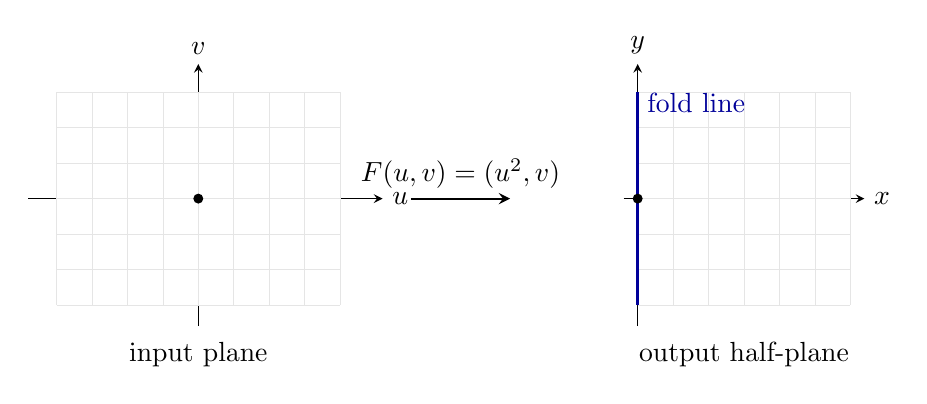
\begin{tikzpicture}[scale=0.9, >=stealth]
    \begin{scope}
        \draw[->] (-2.4,0) -- (2.6,0) node[right] {\(u\)};
        \draw[->] (0,-1.8) -- (0,1.9) node[above] {\(v\)};
        \draw[step=0.5, gray!20, very thin] (-2,-1.5) grid (2,1.5);
        \fill (0,0) circle (2pt);
        \node at (0,-2.2) {input plane};
    \end{scope}

    \draw[->, thick] (3.0,0) -- (4.4,0) node[midway, above] {\(F(u,v)=(u^2,v)\)};

    \begin{scope}[shift={(6.2,0)}]
        \draw[->] (-0.2,0) -- (3.2,0) node[right] {\(x\)};
        \draw[->] (0,-1.8) -- (0,1.9) node[above] {\(y\)};
        \draw[step=0.5, gray!20, very thin] (0,-1.5) grid (3,1.5);

        \draw[very thick, blue!60!black] (0,-1.5) -- (0,1.5);
        \node[blue!60!black, right] at (0,1.35) {fold line};

        \fill (0,0) circle (2pt);
        \node at (1.5,-2.2) {output half-plane};
    \end{scope}
\end{tikzpicture}
\caption{The map \(F(u,v)=(u^2,v)\) folds two sides of the input plane onto the same
output.}
\end{figure}

A zero determinant does not always mean that no inverse exists.  It means the theorem
can no longer guarantee a differentiable inverse.

\begin{example}[An inverse exists, but its derivative blows up]
Let
\[
    F(u,v)=(u^3,v).
\]
This map is one-to-one on the whole plane.  Its inverse is
\[
    F^{-1}(x,y)=(\sqrt[3]{x},y).
\]
But
\[
    J_F(u,v)=
    \begin{pmatrix}
        3u^2 & 0\\
        0 & 1
    \end{pmatrix},
\]
so
\[
    \det J_F(0,0)=0.
\]
The inverse is not differentiable at \((0,0)\), because
\[
    \frac{d}{dx}\sqrt[3]{x}
    =
    \frac{1}{3x^{2/3}}
\]
blows up at \(x=0\).

So the nonzero determinant condition is not saying merely that an inverse exists.  It is
saying that the inverse behaves smoothly and has a linear approximation.
\end{example}

The theorem also asks for continuous first partial derivatives near the point.  A
one-dimensional example shows why some smoothness is needed.

\begin{example}[Why continuity of the derivative is part of the theorem]
Define
\[
    f(t)=
    \begin{cases}
    t+2t^2\sin\left(\dfrac{1}{t^2}\right), & t\ne0,\\[2mm]
    0, & t=0.
    \end{cases}
\]
Then
\[
    f'(0)=1.
\]
So the derivative at the origin is nonzero.

For \(t\ne0\),
\[
    f'(t)=
    1+4t\sin\left(\frac1{t^2}\right)
    -
    \frac4t\cos\left(\frac1{t^2}\right).
\]
The last term oscillates with unbounded size as \(t\to0\).  Thus \(f'\) is not
continuous near \(0\).

In every interval around \(0\), the derivative takes both positive and negative values.
A continuous one-to-one function on an interval must be monotone.  A differentiable
monotone function cannot have derivatives of both signs throughout every tiny interval.
So \(f\) has no local inverse near \(0\), even though
\[
    f'(0)=1.
\]

This example is not meant to be memorized.  Its job is to show that knowing the
derivative at one point is not enough.  The derivative must control a neighborhood.
\end{example}

The inverse function theorem is a local tool.  It says that a map with a non-collapsing
linear part behaves like a coordinate system after enough zooming.

\begin{example}[A nonlinear calibration map]
A small machine has two control variables \((u,v)\), and its output position is modeled by
\[
    F(u,v)=(u+v^2,\ v+u^2).
\]
The Jacobian matrix is
\[
    J_F(u,v)=
    \begin{pmatrix}
        1 & 2v\\
        2u & 1
    \end{pmatrix}.
\]
Its determinant is
\[
    \det J_F(u,v)=1-4uv.
\]

At the origin,
\[
    \det J_F(0,0)=1,
\]
so the inverse function theorem says that \(F\) has a local inverse near \((0,0)\).
Near the origin, we can recover the control values from the output position.

At
\[
    \left(\frac12,\frac12\right),
\]
the determinant is
\[
    1-4\cdot\frac12\cdot\frac12=0.
\]
There the linear approximation is
\[
    J_F\left(\frac12,\frac12\right)
    =
    \begin{pmatrix}
        1 & 1\\
        1 & 1
    \end{pmatrix}.
\]
This matrix sends
\[
    (1,-1)
\]
to
\[
    (0,0).
\]
So, to first order, one input direction is invisible in the output.  The theorem cannot
give a local inverse there.
\end{example}

Solving an inverse problem means recovering all input coordinates from all output
coordinates.  But many problems ask for less.  A curve might be given by one equation
\[
    F(x,y)=0,
\]
and we may only want to solve for \(y\) as a function of \(x\).  A surface might be given
by one equation
\[
    F(x,y,z)=0,
\]
and we may only want to solve for \(z\) as a function of \(x\) and \(y\).  That is not a
full inverse problem.  It is an implicit one.

\section{Implicit functions}
\label{sec:8.6}

An inverse function solves for all inputs from all outputs.  A constraint usually asks for
something smaller.  It gives an equation and asks which points satisfy it.

The unit circle is not usually introduced as
\[
    y=\sqrt{1-x^2}
\]
or
\[
    y=-\sqrt{1-x^2}.
\]
It is introduced as
\[
    x^2+y^2=1.
\]
That equation does not solve for \(y\).  It describes the curve implicitly.

The question is local:

\[
    \text{Near a chosen point, can the equation be solved for one variable?}
\]

\subsection{Curves given by \texorpdfstring{\(F(x,y)=0\)}{F(x,y)=0}}

A pond has an oval shoreline modeled by
\[
    F(x,y)=\frac{x^2}{9}+\frac{y^2}{4}-1=0.
\]
This equation does not choose the upper shore or the lower shore.  It describes both at
once.

Near the top point
\[
    (0,2),
\]
the shoreline is the graph of a function
\[
    y=g(x).
\]
Indeed, solving the equation gives the upper branch
\[
    y=2\sqrt{1-\frac{x^2}{9}}.
\]
Near the bottom point
\[
    (0,-2),
\]
the shoreline is also a graph over \(x\), but with the lower branch
\[
    y=-2\sqrt{1-\frac{x^2}{9}}.
\]

At the rightmost point
\[
    (3,0),
\]
the situation changes.  The shoreline has a vertical tangent.  Near this point, it is not
the graph of \(y\) as a function of \(x\).  For \(x\) slightly less than \(3\), there are two
nearby \(y\)-values, one above and one below the \(x\)-axis.

But it is the graph of \(x\) as a function of \(y\):
\[
    x=3\sqrt{1-\frac{y^2}{4}}.
\]

So the same implicit curve may be solved for different variables at different points.

\begin{figure}[h]
\centering
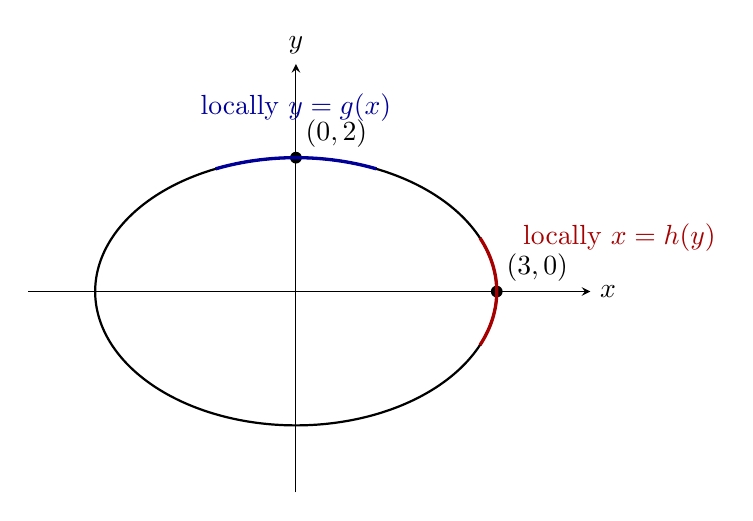
\begin{tikzpicture}[scale=0.85, >=stealth]
    \draw[->] (-4,0) -- (4.4,0) node[right] {\(x\)};
    \draw[->] (0,-3) -- (0,3.4) node[above] {\(y\)};

    \draw[thick, domain=0:360, samples=220, smooth, variable=\t]
        plot ({3*cos(\t)}, {2*sin(\t)});

    \fill (0,2) circle (2.5pt);
    \node[above right] at (0,2) {\((0,2)\)};

    \fill (3,0) circle (2.5pt);
    \node[above right] at (3,0) {\((3,0)\)};

    \draw[very thick, blue!60!black] (-1.2,{2*sqrt(1-1.44/9)})
        arc[start angle=113.6,end angle=66.4,x radius=3,y radius=2];
    \node[blue!60!black] at (0,2.75) {locally \(y=g(x)\)};

    \draw[very thick, red!65!black] ({3*sqrt(1-0.64/4)},-0.8)
        arc[start angle=-23.6,end angle=23.6,x radius=3,y radius=2];
    \node[red!65!black, right] at (3.25,0.8) {locally \(x=h(y)\)};
\end{tikzpicture}
\caption{An implicit curve can be solved for different variables at different points.}
\end{figure}

The partial derivatives of \(F\) predict which variable can be solved for.

For
\[
    F(x,y)=\frac{x^2}{9}+\frac{y^2}{4}-1,
\]
we have
\[
    F_x=\frac{2x}{9},
    \qquad
    F_y=\frac{y}{2}.
\]
At the top point \((0,2)\),
\[
    F_y(0,2)=1\ne0.
\]
That is why we can solve locally for \(y\) as a function of \(x\).

At the rightmost point \((3,0)\),
\[
    F_y(3,0)=0,
\]
so solving for \(y\) is not supported there.  But
\[
    F_x(3,0)=\frac23\ne0,
\]
so solving for \(x\) as a function of \(y\) is supported.

\subsection{Implicit differentiation in the plane}

Suppose a curve is given by
\[
    F(x,y)=0
\]
and, near a point, we can write
\[
    y=g(x).
\]
Then along the curve,
\[
    F(x,g(x))=0.
\]
Differentiate with respect to \(x\):
\[
    F_x(x,g(x))+F_y(x,g(x))g'(x)=0.
\]
So, if
\[
    F_y\ne0,
\]
then
\[
\boxed{
    \frac{dy}{dx}
    =
    -\frac{F_x}{F_y}.
}
\]

The same formula appears even more cleanly with differentials.  Along the curve,
\[
    dF=0.
\]
But
\[
    dF=F_x\,dx+F_y\,dy.
\]
If \(y\) is a function of \(x\), then
\[
    dy=\frac{dy}{dx}\,dx.
\]
Substitute:
\[
    0=F_x\,dx+F_y\frac{dy}{dx}\,dx.
\]
After factoring out \(dx\),
\[
    F_x+F_y\frac{dy}{dx}=0.
\]
Thus
\[
    \frac{dy}{dx}=-\frac{F_x}{F_y}.
\]

\begin{example}[Slope of the oval shoreline]
For the oval
\[
    F(x,y)=\frac{x^2}{9}+\frac{y^2}{4}-1=0,
\]
we found
\[
    F_x=\frac{2x}{9},
    \qquad
    F_y=\frac{y}{2}.
\]
When \(y\ne0\),
\[
    \frac{dy}{dx}
    =
    -\frac{F_x}{F_y}
    =
    -\frac{2x/9}{y/2}
    =
    -\frac{4x}{9y}.
\]
At the top point \((0,2)\),
\[
    \frac{dy}{dx}=0.
\]
At a point on the upper-right part of the shore, such as
\[
    \left(\frac32,\sqrt3\right),
\]
the slope is
\[
    \frac{dy}{dx}
    =
    -\frac{4(3/2)}{9\sqrt3}
    =
    -\frac{2}{3\sqrt3}.
\]
The upper-right shoreline slopes downward as \(x\) increases.
\end{example}

\begin{example}[A nonlinear balance curve]
A chemical balance curve is modeled by
\[
    F(x,y)=xe^y+y-3=0.
\]
The point
\[
    (3,0)
\]
lies on the curve because
\[
    3e^0+0-3=0.
\]
Compute
\[
    F_x=e^y,
\]
and
\[
    F_y=xe^y+1.
\]
At \((3,0)\),
\[
    F_x(3,0)=1,
    \qquad
    F_y(3,0)=4.
\]
Since
\[
    F_y(3,0)\ne0,
\]
the curve can be solved locally as
\[
    y=g(x).
\]
Its slope at \((3,0)\) is
\[
    g'(3)
    =
    -\frac{F_x(3,0)}{F_y(3,0)}
    =
    -\frac14.
\]
\end{example}

\subsection{Surfaces given by \texorpdfstring{\(F(x,y,z)=0\)}{F(x,y,z)=0}}

In space, one equation usually describes a surface.  For example,
\[
    x^2+y^2+z^2=25
\]
describes a sphere of radius \(5\).  The same surface can be written implicitly as
\[
    F(x,y,z)=x^2+y^2+z^2-25=0.
\]

Near a point on the upper hemisphere, where \(z>0\), we can solve for
\[
    z
\]
as a function of \(x\) and \(y\):
\[
    z=\sqrt{25-x^2-y^2}.
\]
Near a point on the lower hemisphere, where \(z<0\), we can also solve for \(z\), but
with the negative branch:
\[
    z=-\sqrt{25-x^2-y^2}.
\]
At the equator, where
\[
    z=0,
\]
we cannot solve the sphere locally as a single graph
\[
    z=g(x,y).
\]
For points \((x,y)\) just inside the equator, there are two nearby \(z\)-values: one
above and one below.

The derivative test sees this.  For
\[
    F(x,y,z)=x^2+y^2+z^2-25,
\]
we have
\[
    F_z=2z.
\]
On the upper and lower hemispheres,
\[
    F_z\ne0.
\]
At the equator,
\[
    F_z=0.
\]
So \(F_z\ne0\) is the condition that supports solving for \(z\).

\subsection{Implicit differentiation in several variables}

Suppose
\[
    F(x,y,z)=0
\]
and near a point we can write
\[
    z=g(x,y).
\]
Then
\[
    F(x,y,g(x,y))=0.
\]
Differentiate with respect to \(x\), holding \(y\) fixed:
\[
    F_x+F_z\,g_x=0.
\]
So
\[
\boxed{
    z_x=g_x=-\frac{F_x}{F_z}.
}
\]
Differentiate with respect to \(y\), holding \(x\) fixed:
\[
    F_y+F_z\,g_y=0.
\]
So
\[
\boxed{
    z_y=g_y=-\frac{F_y}{F_z}.
}
\]
All partial derivatives of \(F\) are evaluated at
\[
    (x,y,z)=(x,y,g(x,y)).
\]

The differential form is shorter.  Along the surface,
\[
    dF=0.
\]
But
\[
    dF=F_x\,dx+F_y\,dy+F_z\,dz.
\]
If
\[
    z=g(x,y),
\]
then
\[
    dz=z_x\,dx+z_y\,dy.
\]
Substitute:
\[
    0=
    F_x\,dx+F_y\,dy+F_z(z_x\,dx+z_y\,dy).
\]
Group the \(dx\) and \(dy\) terms:
\[
    0=(F_x+F_z z_x)\,dx+(F_y+F_z z_y)\,dy.
\]
Since \(dx\) and \(dy\) are independent coordinate changes, both coefficients must
vanish:
\[
    F_x+F_z z_x=0,
    \qquad
    F_y+F_z z_y=0.
\]

\begin{example}[A surface with a mixed term]
Consider the surface
\[
    F(x,y,z)=x^2+y^2+z+xyz-4=0.
\]
The point
\[
    (1,1,1)
\]
lies on the surface because
\[
    1+1+1+1-4=0.
\]
Compute the partial derivatives:
\[
    F_x=2x+yz,
\]
\[
    F_y=2y+xz,
\]
and
\[
    F_z=1+xy.
\]
At \((1,1,1)\),
\[
    F_x=3,
    \qquad
    F_y=3,
    \qquad
    F_z=2.
\]
Since
\[
    F_z\ne0,
\]
the surface can be solved locally as
\[
    z=g(x,y).
\]
The partial derivatives of \(g\) at \((1,1)\) are
\[
    g_x(1,1)=-\frac{F_x}{F_z}=-\frac32,
\]
and
\[
    g_y(1,1)=-\frac{F_y}{F_z}=-\frac32.
\]
So near \((1,1,1)\), the surface has the linear approximation
\[
    z-1
    =
    -\frac32(x-1)-\frac32(y-1).
\]
Equivalently,
\[
\boxed{
    3(x-1)+3(y-1)+2(z-1)=0.
}
\]
This is the tangent plane.
\end{example}

The tangent plane formula is not a separate trick.  It is the equation
\[
    dF=0
\]
applied to a displacement
\[
    (dx,dy,dz)
\]
tangent to the surface:
\[
    F_x\,dx+F_y\,dy+F_z\,dz=0.
\]
At \((a,b,c)\), this becomes
\[
\boxed{
    F_x(a,b,c)(x-a)
    +
    F_y(a,b,c)(y-b)
    +
    F_z(a,b,c)(z-c)
    =
    0.
}
\]
The coefficient vector
\[
    \nabla F(a,b,c)
    =
    (F_x,F_y,F_z)
\]
is normal to the tangent plane.  This observation will become central in Chapter
\ref{ch:9}.

\subsection{The implicit function theorem, stated geometrically}

The examples point to the theorem.

For curves, the rule is:

\[
    F_y\ne0
    \quad\Longrightarrow\quad
    \text{solve locally for }y.
\]

For surfaces, the rule is:

\[
    F_z\ne0
    \quad\Longrightarrow\quad
    \text{solve locally for }z.
\]

\begin{theorem}[Implicit function theorem for a plane curve]
Let
\[
    F(x,y)
\]
have continuous first partial derivatives near \((a,b)\).  Suppose
\[
    F(a,b)=0
\]
and
\[
    F_y(a,b)\ne0.
\]
Then, near \((a,b)\), the equation
\[
    F(x,y)=0
\]
can be solved uniquely as
\[
    y=g(x),
\]
with
\[
    g(a)=b.
\]
The function \(g\) has continuous first derivative, and
\[
\boxed{
    g'(x)=-\frac{F_x(x,g(x))}{F_y(x,g(x))}.
}
\]
In particular,
\[
\boxed{
    g'(a)=-\frac{F_x(a,b)}{F_y(a,b)}.
}
\]
\end{theorem}

If instead
\[
    F_x(a,b)\ne0,
\]
then the equation can be solved locally as
\[
    x=h(y).
\]

\begin{theorem}[Implicit function theorem for a surface]
Let
\[
    F(x,y,z)
\]
have continuous first partial derivatives near \((a,b,c)\).  Suppose
\[
    F(a,b,c)=0
\]
and
\[
    F_z(a,b,c)\ne0.
\]
Then, near \((a,b,c)\), the equation
\[
    F(x,y,z)=0
\]
can be solved uniquely as
\[
    z=g(x,y),
\]
with
\[
    g(a,b)=c.
\]
The function \(g\) has continuous first partial derivatives, and
\[
\boxed{
    g_x=-\frac{F_x}{F_z},
    \qquad
    g_y=-\frac{F_y}{F_z}.
}
\]
The partial derivatives on the right are evaluated at
\[
    (x,y,g(x,y)).
\]
\end{theorem}

\begin{proof}[Why this follows from the inverse function theorem]
For the plane curve theorem, build the map
\[
    \Phi(x,y)=(x,F(x,y)).
\]
Its Jacobian matrix is
\[
    J_\Phi(x,y)
    =
    \begin{pmatrix}
        1 & 0\\
        F_x & F_y
    \end{pmatrix}.
\]
So
\[
    \det J_\Phi(a,b)=F_y(a,b).
\]
If
\[
    F_y(a,b)\ne0,
\]
then \(\Phi\) has a local inverse near \((a,F(a,b))=(a,0)\).

That means the pair
\[
    (x,F(x,y))
\]
can be used as local coordinates near \((a,b)\).  If we set the second coordinate equal
to \(0\), we are looking exactly at points satisfying
\[
    F(x,y)=0.
\]
The inverse of \(\Phi\) then gives
\[
    y=g(x).
\]
The derivative formula comes from differentiating
\[
    F(x,g(x))=0.
\]

For the surface theorem, use
\[
    \Phi(x,y,z)=(x,y,F(x,y,z)).
\]
Its Jacobian determinant is
\[
    F_z(x,y,z).
\]
If
\[
    F_z(a,b,c)\ne0,
\]
the inverse function theorem gives local coordinates
\[
    (x,y,F).
\]
Setting
\[
    F=0
\]
solves the surface locally as
\[
    z=g(x,y).
\]
\end{proof}

\subsection{Why the hypotheses matter}

We required the partial derivative with respect to the variable being solved for to be
nonzero.  Without that condition, uniqueness can fail.

\begin{example}[When \(F_y=0\), \(y\) may not be a function of \(x\)]
Let
\[
    F(x,y)=y^2-x.
\]
The curve
\[
    F(x,y)=0
\]
is
\[
    x=y^2.
\]
At the origin,
\[
    F(0,0)=0,
\]
and
\[
    F_y(x,y)=2y,
\]
so
\[
    F_y(0,0)=0.
\]

For every small positive \(x\), there are two nearby \(y\)-values:
\[
    y=\sqrt{x}
    \qquad\text{and}\qquad
    y=-\sqrt{x}.
\]
So near the origin, the curve is not the graph of one function \(y=g(x)\).

But
\[
    F_x=-1\ne0,
\]
so the same curve can be solved for \(x\) as a function of \(y\):
\[
    x=y^2.
\]
The nonzero partial tells us which variable can be solved for.
\end{example}

We also required smoothness of \(F\).  Without it, the level set may have a corner, and
implicit differentiation may fail.

\begin{example}[A nonsmooth constraint gives a corner]
Let
\[
    F(x,y)=y-|x|.
\]
Then
\[
    F(x,y)=0
\]
is the V-shaped curve
\[
    y=|x|.
\]
At \((0,0)\), this curve is a graph of \(y\) as a function of \(x\), but it is not
differentiable there.  It has a corner.

The partial derivative \(F_x\) does not exist at the origin, because
\[
    |x|
\]
has no derivative at \(0\).  So the formula
\[
    \frac{dy}{dx}=-\frac{F_x}{F_y}
\]
cannot even be formed at the corner.

The smoothness of \(F\) is what prevents this kind of hidden sharp point.
\end{example}

The theorem is also local.  Even when an equation can be solved near a point, it may
not be solvable as one graph over the whole curve.

\begin{example}[One oval, two branches]
For
\[
    \frac{x^2}{9}+\frac{y^2}{4}=1,
\]
the top half is
\[
    y=2\sqrt{1-\frac{x^2}{9}},
\]
and the bottom half is
\[
    y=-2\sqrt{1-\frac{x^2}{9}}.
\]
Most \(x\)-values between \(-3\) and \(3\) give two points on the oval.  So the whole
oval is not one graph \(y=g(x)\), even though each non-vertical part of it is locally a
graph.

Local solvability is the promise.  Global simplicity is not.
\end{example}

The same warning appears for surfaces.

\begin{example}[A sphere cannot be one global height function]
The sphere
\[
    x^2+y^2+z^2=25
\]
has upper and lower halves:
\[
    z=\sqrt{25-x^2-y^2}
\]
and
\[
    z=-\sqrt{25-x^2-y^2}.
\]
Near a point on the upper hemisphere, it is a graph \(z=g(x,y)\).  Near a point on
the lower hemisphere, it is also a graph \(z=g(x,y)\).  At the equator, it is not a
single graph over the \(xy\)-plane, because nearby \((x,y)\)-values inside the equator
give two nearby \(z\)-values.

The equation is smooth.  The failure is caused by
\[
    F_z=2z=0
\]
at the equator.
\end{example}

Implicit equations are not less precise than explicit ones.  They are often more natural.
They describe constraints without choosing a coordinate direction too early.  The
differential
\[
    dF
\]
then tells us the allowed first-order motions:
\[
    dF=0.
\]
That sentence will return soon.  On a constraint, not every direction is available.
A point may be a maximum or minimum not because all motion stops, but because every
\emph{allowed} first-order motion fails to improve the quantity.  That idea leads directly
to gradients, tangent spaces, and constrained optimization.
% Chapter review follows the Chapter 8 outline: review skills, a local-invertibility
% project, and the hook that extrema begin where all first-order changes vanish.
% :contentReference[oaicite:0]{index=0}

\section{Chapter review and discovery problems}
\label{sec:8.7}

Chapter \ref{ch:8} began with one moving point passing through one scalar field:
\[
    t\longmapsto \mathbf r(t)\longmapsto f(\mathbf r(t)).
\]
It ended with implicit surfaces and local coordinates.  The same idea was underneath
all of it:

\[
    \text{first-order changes pass through linear maps.}
\]

Sometimes the linear map was a row vector:
\[
    df=f_x\,dx+f_y\,dy.
\]
Sometimes it was a matrix:
\[
    J_{F\circ G}=J_FJ_G.
\]
Sometimes it was an inverse matrix:
\[
    J_{F^{-1}}=\bigl(J_F\bigr)^{-1}.
\]
Sometimes it was hidden inside an implicit equation:
\[
    dF=0.
\]

This review is meant to make those pieces feel like one machine.

\subsection{The chapter in one picture}

The chain rule is a statement about small changes.  A small input change goes through
one linear approximation, then another.

\begin{figure}[h]
\centering
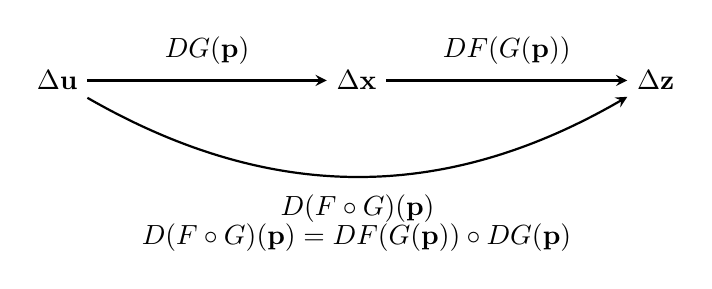
\begin{tikzpicture}[scale=1.0, >=stealth]
    \node (du) at (0,0) {\(\Delta\mathbf u\)};
    \node (dx) at (3.8,0) {\(\Delta\mathbf x\)};
    \node (dz) at (7.6,0) {\(\Delta\mathbf z\)};

    \draw[->, thick] (du) -- (dx)
        node[midway, above=2pt] {\(DG(\mathbf p)\)};
    \draw[->, thick] (dx) -- (dz)
        node[midway, above=2pt] {\(DF(G(\mathbf p))\)};

    \draw[->, thick, bend right=30] (du) to
        node[midway, below=3pt] {\(D(F\circ G)(\mathbf p)\)}
        (dz);

    \node at (3.8,-2.0)
    {\(D(F\circ G)(\mathbf p)=DF(G(\mathbf p))\circ DG(\mathbf p)\)};
\end{tikzpicture}
\caption{The derivative of a composition is the composition of the derivatives.}
\end{figure}

In coordinates, this becomes matrix multiplication:
\[
    J_{F\circ G}(\mathbf p)=J_F(G(\mathbf p))J_G(\mathbf p).
\]
In differential notation, the same idea becomes substitution:
\[
    d(f\circ G)=G^*(df).
\]
The notation changes.  The linear story does not.

\[
\begin{array}{c|c|c}
\text{Situation} & \text{Formula} & \text{Meaning} \\ \hline
\text{field along a curve}
&
\dfrac{d}{dt}f(\mathbf r(t))
=
\nabla f(\mathbf r(t))\cdot\mathbf r'(t)
&
\text{rate seen by a moving observer}
\\[3mm]
\text{composition of maps}
&
J_{F\circ G}=J_FJ_G
&
\text{linearize, then compose}
\\[3mm]
\text{differentials}
&
df=f_x\,dx+f_y\,dy
&
\text{best linear change in }f
\\[3mm]
\text{coordinate change}
&
dx\wedge dy=
\dfrac{\partial(x,y)}{\partial(u,v)}\,du\wedge dv
&
\text{local signed area scaling}
\\[4mm]
\text{inverse map}
&
J_{F^{-1}}=
(J_F)^{-1}
&
\text{reverse the linear approximation}
\\[3mm]
\text{implicit curve or surface}
&
dF=0
&
\text{allowed first-order motions stay on the constraint}
\end{array}
\]

\subsection{Worked review example: a moving thermometer}

Let
\[
    S(x,y,z)=12+xz-y^2
\]
be a salinity field in a tank.  A probe moves along
\[
    \mathbf r(t)=(1+t,\;2-t^2,\;3e^t).
\]
Find the rate of change of salinity seen by the probe at \(t=0\).

The probe starts at
\[
    \mathbf r(0)=(1,2,3).
\]
Its velocity is
\[
    \mathbf r'(t)=(1,-2t,3e^t),
\]
so
\[
    \mathbf r'(0)=(1,0,3).
\]
The gradient of \(S\) is
\[
    \nabla S(x,y,z)=(z,-2y,x).
\]
At the starting point,
\[
    \nabla S(1,2,3)=(3,-4,1).
\]
Therefore
\[
\begin{aligned}
    \frac{d}{dt}S(\mathbf r(t))\bigg|_{t=0}
    &=
    \nabla S(1,2,3)\cdot\mathbf r'(0)\\
    &=
    (3,-4,1)\cdot(1,0,3)\\
    &=
    6.
\end{aligned}
\]
The probe sees salinity increasing at rate \(6\) salinity units per second.

The calculation can also be read as
\[
    dS_{\mathbf r(0)}\bigl(\mathbf r'(0)\bigr)=6.
\]
The differential \(dS\) eats the velocity vector and returns the observed rate.

\subsection{Worked review example: a matrix chain rule calculation}

Let
\[
    G(u,v)=(u^2+v,\;e^u-v),
\]
and let
\[
    F(x,y)=(xy,\;x+y^2).
\]
Set
\[
    H=F\circ G.
\]
Find
\[
    J_H(0,1)
\]
without expanding \(H\).

First compute the intermediate point:
\[
    G(0,1)=(1,0).
\]
The Jacobian matrix of \(G\) is
\[
    J_G(u,v)=
    \begin{pmatrix}
        2u & 1\\
        e^u & -1
    \end{pmatrix},
\]
so
\[
    J_G(0,1)=
    \begin{pmatrix}
        0 & 1\\
        1 & -1
    \end{pmatrix}.
\]

The Jacobian matrix of \(F\) is
\[
    J_F(x,y)=
    \begin{pmatrix}
        y & x\\
        1 & 2y
    \end{pmatrix}.
\]
At \((x,y)=(1,0)\),
\[
    J_F(1,0)=
    \begin{pmatrix}
        0 & 1\\
        1 & 0
    \end{pmatrix}.
\]
Therefore
\[
\begin{aligned}
    J_H(0,1)
    &=
    J_F(G(0,1))J_G(0,1)\\
    &=
    \begin{pmatrix}
        0 & 1\\
        1 & 0
    \end{pmatrix}
    \begin{pmatrix}
        0 & 1\\
        1 & -1
    \end{pmatrix}\\
    &=
    \begin{pmatrix}
        1 & -1\\
        0 & 1
    \end{pmatrix}.
\end{aligned}
\]

The order matters.  A small \((u,v)\)-change first passes through \(G\), and only then
through \(F\).  That is why the matrix for \(G\) stands on the right.

\subsection{Worked review example: area scaling from differentials}

Let a coordinate change be given by
\[
    x=s^2-t,
    \qquad
    y=s+t^2.
\]
Find the local signed area factor.

Differentiate:
\[
    dx=2s\,ds-dt,
\]
and
\[
    dy=ds+2t\,dt.
\]
Then
\[
\begin{aligned}
dx\wedge dy
&=
(2s\,ds-dt)\wedge(ds+2t\,dt)\\
&=
4st\,ds\wedge dt-dt\wedge ds\\
&=
4st\,ds\wedge dt+ds\wedge dt\\
&=
(4st+1)\,ds\wedge dt.
\end{aligned}
\]
Thus
\[
\boxed{
    \frac{\partial(x,y)}{\partial(s,t)}=4st+1.
}
\]

At points where
\[
    4st+1\ne0,
\]
the coordinate change does not collapse tiny areas.  The inverse function theorem says
that the map has a local inverse there.

At points where
\[
    4st+1=0,
\]
tiny signed area is collapsed to first order.  The theorem no longer promises a local
inverse.

The same number comes from the determinant:
\[
\det
\begin{pmatrix}
    x_s & x_t\\
    y_s & y_t
\end{pmatrix}
=
\det
\begin{pmatrix}
    2s & -1\\
    1 & 2t
\end{pmatrix}
=
4st+1.
\]

\subsection{Worked review example: an implicit surface}

Consider the surface
\[
    F(x,y,z)=x^2+yz+z^2-3=0.
\]
The point
\[
    (1,1,1)
\]
lies on the surface because
\[
    1+1+1-3=0.
\]
Can the surface be solved near this point as
\[
    z=g(x,y)?
\]
If so, find \(g_x(1,1)\), \(g_y(1,1)\), and the tangent plane.

Compute
\[
    F_x=2x,
    \qquad
    F_y=z,
    \qquad
    F_z=y+2z.
\]
At \((1,1,1)\),
\[
    F_z(1,1,1)=3\ne0.
\]
So the implicit function theorem says that the surface can be solved locally as
\[
    z=g(x,y).
\]
The partial derivatives are
\[
    g_x=-\frac{F_x}{F_z},
    \qquad
    g_y=-\frac{F_y}{F_z}.
\]
Therefore
\[
    g_x(1,1)=-\frac23,
    \qquad
    g_y(1,1)=-\frac13.
\]

The tangent plane is
\[
    F_x(1,1,1)(x-1)
    +
    F_y(1,1,1)(y-1)
    +
    F_z(1,1,1)(z-1)
    =
    0.
\]
So
\[
\boxed{
    2(x-1)+(y-1)+3(z-1)=0.
}
\]

The same answer comes from
\[
    dF=0.
\]
At the point,
\[
    dF=2\,dx+dy+3\,dz.
\]
A first-order motion tangent to the surface must satisfy
\[
    2\,dx+dy+3\,dz=0.
\]

\subsection{Concept check}

\begin{enumerate}
\item What is the difference between a partial derivative and a total derivative?

\item In the formula
\[
    \frac{d}{dt}f(\mathbf r(t))
    =
    \nabla f(\mathbf r(t))\cdot\mathbf r'(t),
\]
where is the gradient evaluated?

\item Why is
\[
    J_{F\circ G}=J_FJ_G
\]
not the same as
\[
    J_GJ_F?
\]

\item What does the formula
\[
    dx=x_u\,du+x_v\,dv
\]
mean geometrically?

\item When we pull back a \(1\)-form
\[
    \omega=P(x,y)\,dx+Q(x,y)\,dy
\]
by a map
\[
    G(u,v)=(x(u,v),y(u,v)),
\]
what must be substituted?

\item In polar coordinates, why is
\[
    F_\theta
\]
a rate per radian rather than a rate per meter?

\item What does the Jacobian determinant measure locally?

\item Why does
\[
    \det J_F(\mathbf p)\ne0
\]
give only a local inverse, not necessarily a global inverse?

\item If
\[
    F(x,y)=0
\]
and
\[
    F_y(a,b)\ne0,
\]
which variable can be solved for near \((a,b)\)?

\item If
\[
    F(x,y,z)=0
\]
and
\[
    F_z(a,b,c)\ne0,
\]
what are the formulas for \(z_x\) and \(z_y\)?

\item What does the equation
\[
    dF=0
\]
say about first-order motions along the constraint \(F=0\)?

\item Give an example of a map whose Jacobian determinant is nonzero everywhere but
which is not one-to-one globally.
\end{enumerate}

\subsection{Skill problems}

\begin{enumerate}
\item Let
\[
    f(x,y)=x^2y+\sin y,
    \qquad
    \mathbf r(t)=\left(1+t^2,\frac{\pi}{2}-t\right).
\]
Find
\[
    \frac{d}{dt}f(\mathbf r(t))\bigg|_{t=0}.
\]

\item Let
\[
    T(x,y,z)=xy+z^2-xz,
\]
and
\[
    \mathbf r(t)=(e^t,1-t,2+t^2).
\]
Find the rate of change of \(T\) along \(\mathbf r\) at \(t=0\).

\item A field \(f(x,y,z)\) has
\[
    \nabla f(2,1,0)=(4,-1,3).
\]
A particle passes through \((2,1,0)\) with velocity
\[
    (1,2,-2).
\]
Find the rate at which the particle sees \(f\) change.

\item Let
\[
    z=f(x,y),
    \qquad
    x=u^2+v,
    \qquad
    y=u-v^2.
\]
Write formulas for
\[
    z_u
    \qquad\text{and}\qquad
    z_v.
\]

\item Let
\[
    w=f(x,y,z),
\]
where
\[
    x=uv,\qquad y=u+v,\qquad z=u^2-v^2.
\]
Write formulas for
\[
    w_u
    \qquad\text{and}\qquad
    w_v.
\]

\item Let
\[
    G(u,v)=(u+v,\;uv),
\]
and
\[
    F(x,y)=(x^2+y,\;xy).
\]
Find
\[
    J_{F\circ G}(1,2)
\]
using the matrix chain rule.

\item Let
\[
    G(s,t)=(s^2+t,\;s-t^2,\;st),
\]
and
\[
    F(x,y,z)=x+y^2-z.
\]
Find the row matrix
\[
    J_{F\circ G}(1,1).
\]

\item Let
\[
    u=x^2+y,
    \qquad
    v=x-y^2.
\]
Find
\[
    du
    \qquad\text{and}\qquad
    dv.
\]

\item Let
\[
    f(x,y)=e^{xy}.
\]
Use differentials to compute \(d(f\circ G)\), where
\[
    G(u,v)=(u+v,\;u-v).
\]

\item Pull back the \(1\)-form
\[
    \omega=x\,dy-y\,dx
\]
by the map
\[
    x=u^2,\qquad y=v^2.
\]

\item Pull back the area form
\[
    dx\wedge dy
\]
under
\[
    x=u+v,
    \qquad
    y=u^2-v.
\]
Where does the map collapse signed area to first order?

\item In polar coordinates,
\[
    x=r\cos\theta,
    \qquad
    y=r\sin\theta.
\]
Let
\[
    f(x,y)=x^2-3y.
\]
Find
\[
    F_r
    \qquad\text{and}\qquad
    F_\theta
\]
for
\[
    F(r,\theta)=f(r\cos\theta,r\sin\theta).
\]

\item Let
\[
    f(x,y)=xy.
\]
Write \(f\) in polar coordinates and find the tangential rate per meter at
\[
    r=2,\qquad \theta=\frac{\pi}{4}.
\]

\item In cylindrical coordinates, write
\[
    p(x,y,z)=x^2+y^2-z
\]
as a function
\[
    P(r,\theta,z).
\]
Find
\[
    P_r,\qquad P_\theta,\qquad P_z.
\]

\item In spherical coordinates,
\[
    x=\rho\sin\phi\cos\theta,
    \qquad
    y=\rho\sin\phi\sin\theta,
    \qquad
    z=\rho\cos\phi.
\]
Write
\[
    x^2+y^2+z^2
\]
in spherical coordinates, and explain why its \(\theta\)- and \(\phi\)-derivatives vanish.

\item Let
\[
    F(u,v)=(u+v^2,\;v-u^2).
\]
Find
\[
    \det J_F(u,v).
\]
At which points does the inverse function theorem guarantee a local inverse?

\item Let
\[
    F(u,v)=(e^u\cos v,e^u\sin v).
\]
Find
\[
    \det J_F(u,v).
\]
Explain why \(F\) has local inverses everywhere but no global inverse on all of
\(\mathbb R^2\).

\item Suppose
\[
    F(1,2)=(4,5)
\]
and
\[
    J_F(1,2)=
    \begin{pmatrix}
        2 & 1\\
        1 & 1
    \end{pmatrix}.
\]
If \(G=F^{-1}\) locally near \((4,5)\), find
\[
    J_G(4,5).
\]

\item Let
\[
    F(x,y)=x^3+y^3-6xy.
\]
At the point \((3,3)\), can the curve \(F(x,y)=0\) be solved locally as
\[
    y=g(x)?
\]
If so, find \(g'(3)\).

\item Let
\[
    F(x,y)=x^2-y^2.
\]
At \((0,0)\), can the equation \(F(x,y)=0\) be solved locally as one function
\(y=g(x)\)?  Explain.

\item Let
\[
    F(x,y,z)=x^2+y^2+z^2-9.
\]
Find where the sphere can be solved locally as
\[
    z=g(x,y).
\]
At such points, find \(z_x\) and \(z_y\).

\item Let
\[
    F(x,y,z)=x+y+z+xyz-4.
\]
At \((1,1,1)\), solve locally for \(z=g(x,y)\) and find
\[
    g_x(1,1),
    \qquad
    g_y(1,1).
\]

\item Find the tangent plane to
\[
    x^2+2y^2+3z^2=12
\]
at
\[
    (1,2,1).
\]

\item Let
\[
    F(x,y,u,v)=x+u^2+v-3,
\]
and
\[
    G(x,y,u,v)=y+u-v^2-1.
\]
At
\[
    (x,y,u,v)=(1,1,1,1),
\]
show that the system
\[
    F=0,\qquad G=0
\]
can be solved locally for \(u\) and \(v\) as functions of \(x\) and \(y\).

\item For the system in the previous problem, find
\[
    \frac{\partial u}{\partial x}
    \qquad\text{and}\qquad
    \frac{\partial v}{\partial x}
\]
at \((x,y)=(1,1)\).

\item Give an example of a function whose partial derivatives exist at a point but which
is not differentiable there.  Explain why the chain rule cannot be trusted at that point.
\end{enumerate}

\subsection{Discovery project: local invertibility of a nonlinear map}

A rubber sheet is marked with coordinates \((u,v)\).  A machine sends each marked
point to a new point
\[
    F(u,v)=(x,y)
\]
according to
\[
\boxed{
    x=u+v^2,\qquad y=v+u^2.
}
\]
This map is close to the identity near the origin, but it folds near another point.

The goal of the project is to locate the fold and connect it to the Jacobian determinant.

\subsubsection*{Part 1. The first-order test}

Compute the Jacobian matrix:
\[
    J_F(u,v)=
    \begin{pmatrix}
        x_u & x_v\\
        y_u & y_v
    \end{pmatrix}.
\]
Show that
\[
\boxed{
    J_F(u,v)=
    \begin{pmatrix}
        1 & 2v\\
        2u & 1
    \end{pmatrix}
}
\]
and
\[
\boxed{
    \det J_F(u,v)=1-4uv.
}
\]

The inverse function theorem says that \(F\) has a local inverse at every point where
\[
    1-4uv\ne0.
\]
So the only possible trouble occurs on the hyperbola
\[
    uv=\frac14.
\]

\begin{figure}[h]
\centering
\begin{tikzpicture}[scale=1.0, >=stealth]
    \draw[->] (-3.2,0) -- (3.3,0) node[right] {\(u\)};
    \draw[->] (0,-3.2) -- (0,3.3) node[above] {\(v\)};

    \draw[domain=0.12:3, samples=120, smooth, thick, blue!60!black]
        plot (\x,{1/(4*\x)});
    \draw[domain=-3:-0.12, samples=120, smooth, thick, blue!60!black]
        plot (\x,{1/(4*\x)});

    \fill (0.5,0.5) circle (2.5pt);
    \node[above right] at (0.5,0.5) {\(\left(\frac12,\frac12\right)\)};

    \node[blue!60!black] at (2.1,0.8) {\(uv=\frac14\)};
    \node at (0,-3.8) {The determinant vanishes on the fold curve.};
\end{tikzpicture}
\caption{The curve \(uv=\frac14\) is where the linear approximation collapses area.}
\end{figure}

\subsubsection*{Part 2. The wedge-product version}

Use
\[
    x=u+v^2,
    \qquad
    y=v+u^2
\]
to compute
\[
    dx
    \qquad\text{and}\qquad
    dy.
\]
Then show that
\[
\boxed{
    dx\wedge dy=(1-4uv)\,du\wedge dv.
}
\]
This says that the determinant is not only a matrix number.  It is the coefficient that
tells how signed area forms transform.

\subsubsection*{Part 3. Near the origin}

At the origin,
\[
    J_F(0,0)=
    \begin{pmatrix}
        1 & 0\\
        0 & 1
    \end{pmatrix}.
\]
So near the origin,
\[
    F(u,v)
\]
looks like the identity map.

The inverse function theorem gives a local inverse near
\[
    F(0,0)=(0,0).
\]
To first order,
\[
    u\approx x,
    \qquad
    v\approx y.
\]

A better second-order approximation can be guessed from the equations
\[
    x=u+v^2,
    \qquad
    y=v+u^2.
\]
Since near the origin \(u\approx x\) and \(v\approx y\), substitute those first guesses
into the squared terms:
\[
    u\approx x-y^2,
    \qquad
    v\approx y-x^2.
\]
Check this approximation by substituting
\[
    u=x-y^2,
    \qquad
    v=y-x^2
\]
back into \(F\), and keep only terms up to second degree.

\subsubsection*{Part 4. The fold at \texorpdfstring{\(\left(\frac12,\frac12\right)\)}{(1/2,1/2)}}

At
\[
    \left(\frac12,\frac12\right),
\]
the Jacobian matrix is
\[
    J_F\left(\frac12,\frac12\right)
    =
    \begin{pmatrix}
        1 & 1\\
        1 & 1
    \end{pmatrix}.
\]
This matrix sends
\[
    (1,-1)
\]
to
\[
    (0,0).
\]
So, to first order, motion in the direction \((1,-1)\) is invisible.

Now look at this line through the point:
\[
    (u,v)=\left(\frac12+s,\frac12-s\right).
\]
Compute:
\[
\begin{aligned}
F\left(\frac12+s,\frac12-s\right)
&=
\left(
\frac12+s+\left(\frac12-s\right)^2,\;
\frac12-s+\left(\frac12+s\right)^2
\right)\\
&=
\left(
\frac34+s^2,\;
\frac34+s^2
\right).
\end{aligned}
\]
The same formula holds for \(-s\):
\[
F\left(\frac12+s,\frac12-s\right)
=
F\left(\frac12-s,\frac12+s\right).
\]
So every tiny neighborhood of
\[
    \left(\frac12,\frac12\right)
\]
contains two different points that map to the same output.  There is no local inverse
there.

This is the nonlinear fold that the zero determinant was warning us about.

\subsubsection*{What to hand in}

Write a short report with the following pieces.

\begin{enumerate}
\item The Jacobian matrix and determinant of \(F\).

\item The wedge-product computation
\[
    dx\wedge dy=(1-4uv)\,du\wedge dv.
\]

\item A drawing of the curve
\[
    uv=\frac14
\]
in the \((u,v)\)-plane.

\item A paragraph explaining why the inverse function theorem applies away from that
curve.

\item The exact calculation showing that the two points
\[
    \left(\frac12+s,\frac12-s\right)
    \quad\text{and}\quad
    \left(\frac12-s,\frac12+s\right)
\]
have the same image.

\item A short explanation of how the determinant, the area form, and the visible fold are
three views of the same event.
\end{enumerate}

\subsection{End-of-chapter hook: where first-order motion goes silent}

The chapter kept asking what a function does to first-order changes.  A curve feeds a
velocity into a differential.  A coordinate change feeds one area form into another.  An
implicit surface keeps only the motions that satisfy
\[
    dF=0.
\]

Now imagine a new question.  A hiker stands on a hill and wants the highest nearby
point.  If every tiny step in some direction changes the height to first order, then one of
those steps must improve the height.  So at an interior maximum or minimum, something
strange has to happen:
\[
    df
\]
must vanish on every possible first-order motion.

For a free point in the plane, that becomes
\[
    \nabla f=\mathbf 0.
\]
For a point constrained to a curve or surface, only some motions are allowed, and the
same sentence becomes more subtle.  The steepest direction may point off the constraint
entirely.

That is where optimization begins: not with a formula for the largest value, but with the
silence of all first-order changes.

